\documentclass[a4paper]{report}
\usepackage[utf8]{inputenc}
\usepackage[italian]{babel}
\usepackage[pdftex]{hyperref}
\usepackage{graphicx}
\usepackage{listings}
\usepackage{multirow}
\usepackage{pdflscape}
\usepackage{tabularx}

\hypersetup{
	breaklinks,
	colorlinks,
	linkcolor=blue,
	pdftitle={Relazione},
	pdfsubject={FORSE - Relazione sul progetto di Sistemi Concorrenti e Distribuiti},
	pdfauthor={Daniele Battaglia \& Davide Pesavento}
}

\title{{\huge \textsl{F.O.R.S.E.}}\\
	{\large Relazione sul progetto di Sistemi Concorrenti e Distribuiti}}
\author{Daniele Battaglia\\\url{dbat.fk@gmail.com}
	\and Davide Pesavento\\\url{davidepesa@gmail.com}}
%\date{}

\newcommand{\term}[2]{\textbf{#1} & #2 \\ \\}
\newcommand{\Erlang}{\textsl{Erlang}}
\newcommand{\Python}{\textsl{Python}}
\newcommand{\fun}[1]{\texttt{#1}}


\begin{document}

\maketitle

\tableofcontents

\listoffigures

\clearpage


\chapter{Introduzione}
La presente relazione, unitamente al software denominato \textsl{``Formula One Race Simulation Engine''} (\textsl{FORSE}), è stata realizzata come prova d'esame per il corso ``Sistemi Concorrenti e Distribuiti''.

I requisiti considerati in fase di progettazione sono stati ricavati da quelli proposti dal docente\footnote{\url{http://www.math.unipd.it/~tullio/SCD/2008/Progetto.html}} secondo le clausole di partecipazione di livello 3.

\textsl{FORSE} è stato realizzato utilizzando i linguaggi di programmazione \Erlang{} e \Python{}. Per la distribuzione dell'applicazione abbiamo
usato il protocollo di distribuzione \Erlang{}, supportato nativamente dall'omonimo linguaggio e implementato dalla libreria \textsl{TwOTP} per il linguaggio
\Python{}.
Per la creazione di interfacce grafiche è stata utilizzata la libreria \textsl{Qt}.

Nelle fasi di progettazione e realizzazione del prototipo è stata posta maggiore attenzione riguardo le tematiche inerenti distribuzione e concorrenza, nozioni
centrali del corso, a scapito della parte riguardante la correttezza della simulazione da un punto di vista fisico. Abbiamo comunque cercato di includere
gli elementi essenziali della dinamica di una gara automobilistica anche se con alcune semplificazioni.

Nella prima parte del documento verranno esposti i requisiti espliciti, ricavati dalle richieste del docente, ed impliciti, estratti dal contesto reale che il software \textsl{FORSE} deve simulare.
In seguito verranno elencati i problemi intrinseci che la progettazione del sistema deve affrontare ed essi verranno analizzati alla luce delle conoscenze acquisite durante il corso.
Nella seconda parte della relazione verrà illustrata la nostra soluzione, prima a livello progettuale/architetturale e successivamente a livello di implementazione, mostrando come i problemi precedentemente individuati vengano risolti in modo soddisfacente dal prototipo.


\chapter{Requisiti}
\begin{enumerate}
\item Il sistema deve essere composto da più entità concorrenti e distribuite su una rete.
\item La simulazione evolve in modo deterministico.
\item Il circuito è suddiviso in settori ed è configurabile dall'utente tramite file di configurazione. L'utente deve poter specificare le seguenti informazioni:
	\begin{itemize}
	\item tipo di settore (rettilineo, curvilineo, entrata e uscita dai \textit{box}, intermedio cronometrico, traguardo);
	\item lunghezza e larghezza di ciascun settore;
	\item se il settore è una curva, direzione (destra o sinistra) e raggio di curvatura;
	\item pendenza del suolo;
	\item tempo atmosferico iniziale;
	\item eventuali variazioni del tempo atmosferico nel corso della gara.
	\end{itemize}
\item Insieme configurabile di concorrenti aventi le seguenti caratteristiche:
	\begin{itemize}
	\item nome;
	\item scuderia di appartenenza;
	\item esperienza/bravura;
	\item peso;
	\item vettura utilizzata.
	\end{itemize}
\item Parametri di configurazione delle auto:
	\begin{itemize}
	\item capienza del serbatoio;
	\item quantità di carburante presente nel serbatoio ad inizio gara;
	\item tipo dei pneumatici montati ad inizio gara (\textit{slick}, intermedi, da bagnato);
	\item potenza del motore;
	\item potenza dei freni;
	\item peso a secco.
	\end{itemize}
\item Parametri di configurazione di una competizione:
	\begin{itemize}
	\item numero totale di giri da effettuare;
	\item opzionalmente, la posizione dei concorrenti sulla griglia di partenza;
	\end{itemize}
\item Il sistema di controllo deve essere composto da:
	\begin{itemize}
	\item un pannello generale indicante posizione dei concorrenti in gara, tempi di percorrenza attuali e miglior tempo sul giro, con la possibilità per l'utente di sospendere e riprendere la simulazione;
	\item situazione atmosferica della pista, con la possibilità per l'utente di apportare modifiche alle condizioni meteo anche dopo che la gara è iniziata;
	\item un pannello per ciascuna scuderia che riporta i parametri tecnici rilevanti delle vetture dei propri piloti (carburante residuo, mescola dei pneumatici e loro condizioni di usura) nonché i tempi di percorrenza per settore di pista e totali; deve essere inoltre possibile per l'utente forzare la sosta ai box e il ritiro di un'auto.
	\end{itemize}
\end{enumerate}


\chapter{Problematiche di progettazione}

In questo capitolo verranno individuati i principali problemi incontrati nella progettazione del sistema, sia a livello di coordinazione delle componenti distribuite, sia a livello di meccaniche di simulazione.

\subsection*{Avvio del sistema}
La simulazione non può iniziare finché tutte le componenti necessarie non siano state avviate correttamente e siano pronte all'esecuzione. Per esempio la gara non deve iniziare prima che tutte le auto e le scuderie che vi partecipano siano pronte e correttamente inizializzate, altrimenti si potrebbero avere delle inconsistenze nella simulazione. In sostanza, è necessario implementare una barriera per la sincronizzazione di questi processi necessari alla simulazione.

\subsection*{Accesso alla pista}
Le modifiche alle condizioni della pista devono essere eseguite in mutua esclusione per evitare inconsistenze nel suo stato interno, è necessario quindi che i processi che accedono alle informazioni sulla pista eseguano in modo ordinato e solo quando previsto dalla logica di simulazione. In particolare non deve accadere che due auto effettuino contemporaneamente uno spostamento oppure che vengano modificate le condizioni atmosferiche mentre un'auto si sta muovendo sul tracciato.
La concorrenza deve quindi essere controllata per evitare queste situazioni di \textit{race condition}.

\subsection*{Sorpassi coerenti}
Quando due auto si trovano a percorrere lo stesso segmento di pista devono interagire in modo realistico. Devono essere quindi chiare e verosimili le condizioni che permettono ad un'auto di sorpassarne un'altra, per evitare che si verifichino sorpassi dove la pista o la presenza di altre auto non lo consentano.

\subsection*{Comunicazione di sosta}
Un'auto effettua il rifornimento solo quando richiesto da un attore esterno. Questo attore può essere la propria scuderia o l'utente.

La scuderia indica all'auto durante quale giro di gara effettuare la sosta in base alle informazioni raccolte sulle \textit{performance} dell'auto stessa, di conseguenza è possibile che, al variare delle condizioni della pista, la scuderia calcoli una nuova strategia. Nel caso di un cambiamento delle condizioni atmosferiche, per esempio, la scuderia può decidere di far rientrare ai \textit{box} un'auto al fine di montare dei pneumatici adeguati alle nuove condizioni. Risulta quindi evidente che il messaggio usato dalla scuderia per comunicare all'auto in che giro effettuare la sosta successiva può essere inviato più volte e l'auto deve tenere in considerazione solo quello più recente.

L'utente può invece forzare la sosta immediata di un'auto ai \textit{box}. L'interazione con l'utente avviene in modo asincrono rispetto alla simulazione e deve avere la precedenza sulle direttive provenienti dalla scuderia.

Le situazioni da evitare sono quindi due:
\begin{itemize}
\item Un'auto effettua una sosta ai \textit{box} sulla base di informazioni non aggiornate,
\item La richiesta di sosta proveniente dall'utente viene ignorata a causa di una successiva ricezione di direttive diverse dalla scuderia.
\end{itemize}

\subsection*{Variazione condizioni atmosferiche}
Le variazioni alle condizioni atmosferiche sono effettuate dal sistema in modo sincrono alla competizione nel caso in cui siano state previste a livello di configurazione oppure possono avvenire a seguito di un intervento dell'utente in modo asincrono rispetto alla competizione. Il sistema deve quindi permettere di effettuare queste modifiche evitando i problemi di \textit{race condition} precedentemente evidenziati.

\subsection*{Realismo}
Poiché il prototipo deve simulare una situazione reale, si è reso necessario trovare un \textit{trade-off} adeguato tra la semplicità di implementazione e l'accuratezza della simulazione. Questo vale sia dal punto di vista delle leggi fisiche a cui sono soggette le auto nel percorrere un segmento, sia dal punto di vista della rappresentazione della pista e delle sue regole di percorrenza. Nella realtà per esempio due auto appartenenti alla stessa scuderia non possono effettuare il rifornimento in contemporanea e devono rispettare i limiti di velocità imposti dal regolamento quando si trovano nella \textit{pit lane}.

\subsection*{Fine della competizione}
Il sistema deve essere in grado di riconoscere la fine della competizione ovvero quando l'ultima auto in gara taglia il traguardo. In risposta a questo evento il sistema deve reagire in modo opportuno, mettendosi in uno stato che impedisca alla simulazione di procedere inutilmente.

Deve essere quindi previsto un modo per comunicare a tutte le componenti del sistema di terminare la propria esecuzione, nel caso in cui non servano più, oppure di mettersi in uno stato di sospensione per permettere all'utente di consultare i dati raccolti durante la simulazione.


\chapter{Architettura del sistema}
In questa sezione verranno descritte a livello funzionale le varie componenti del sistema e classificate secondo il modello visto a lezione.

In figura~\ref{fig:architettura} è riportata una vista architetturale ad alto livello del sistema. La figura non riporta tutta le componenti del sistema per non renderne difficile la fruizione. E' stata infatti omessa tutta la parte riguardate l'invio di messaggi dalla componente \texttt{event\_dispatcher} verso il resto del sistema, in quanto trattata in dettaglio nella sezione~\ref{sec:event_dispatcher}.

Vengono inoltre omesse nello schema le componenti riguardati l'inizializzazione del prototipo descritte invece in dettaglio nella sezione~\ref{sec:start-stop}.
\begin{landscape}
\begin{figure}
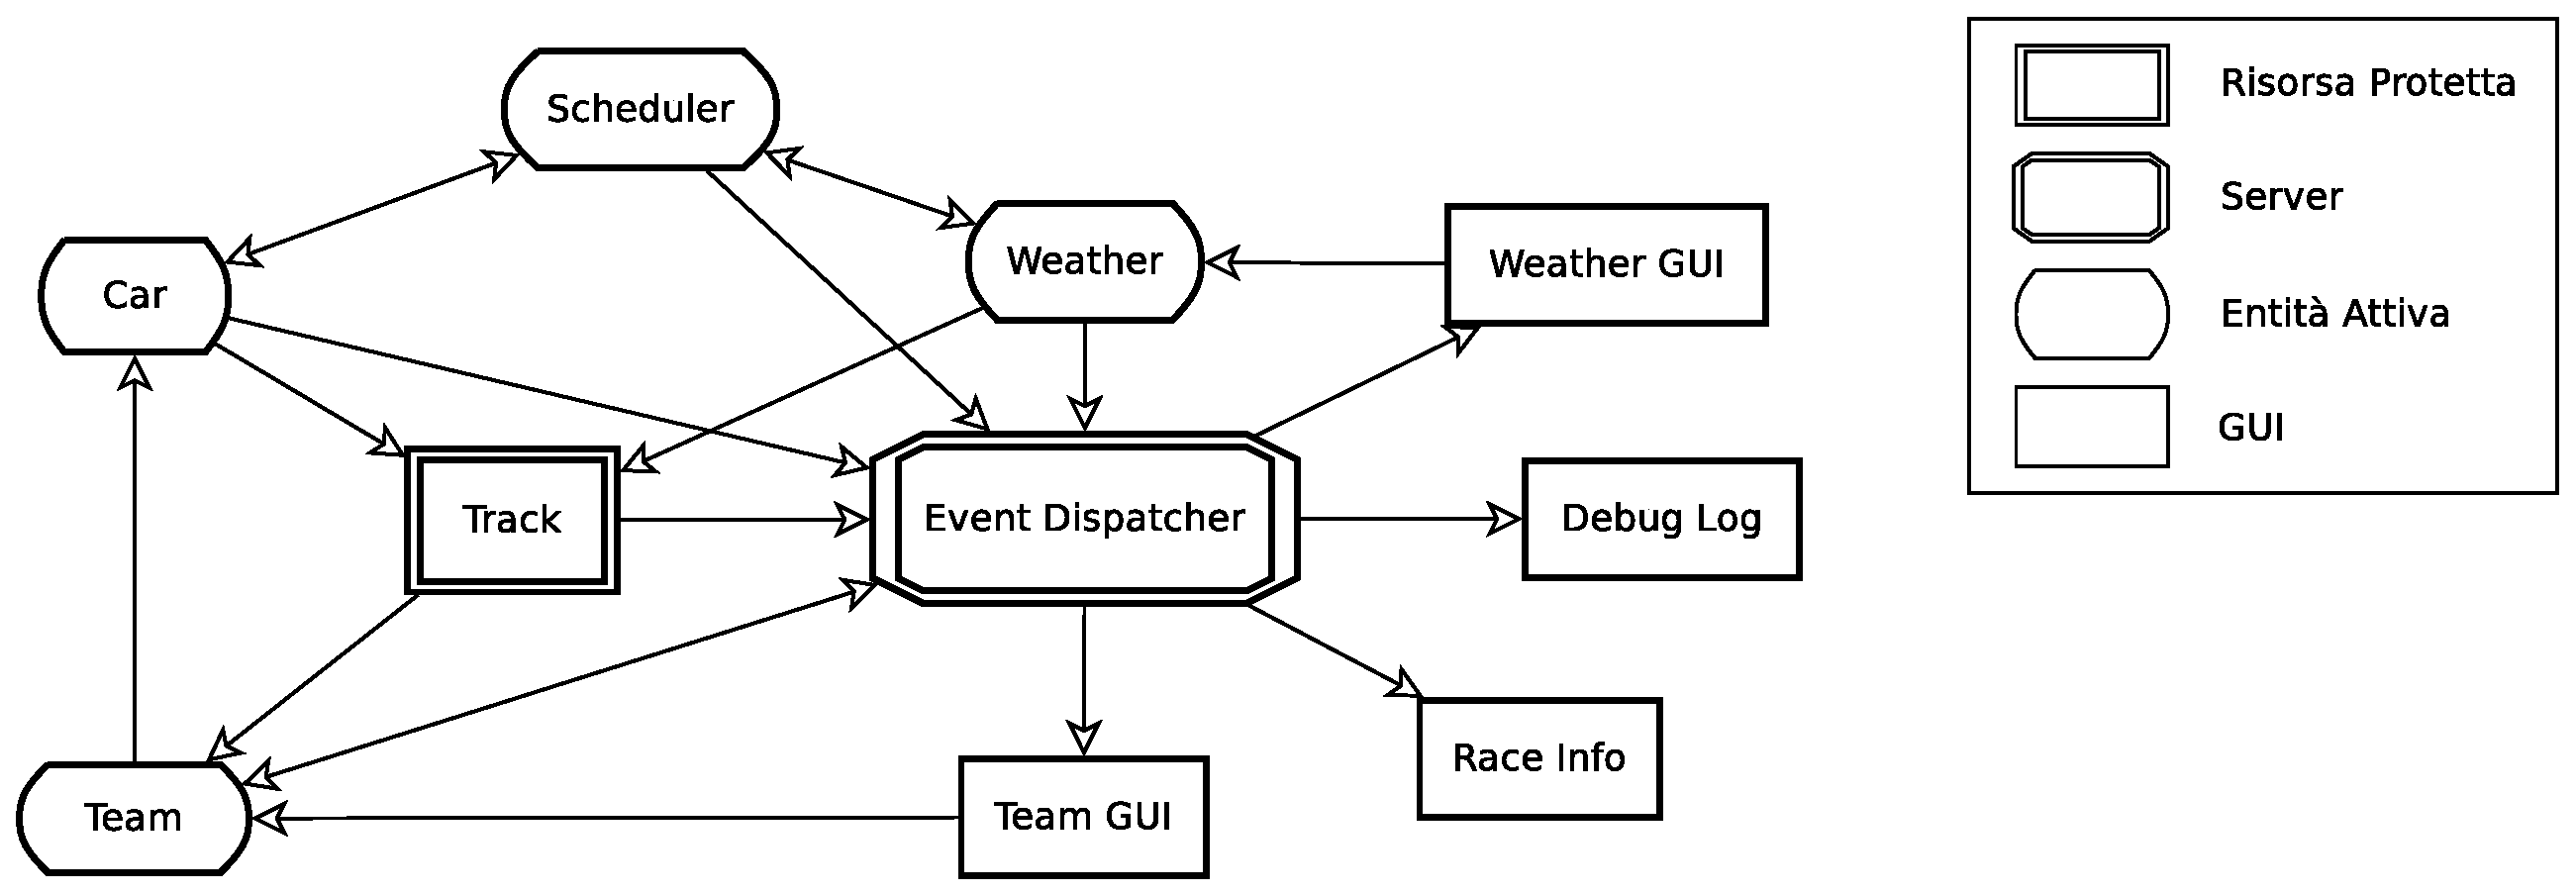
\includegraphics[height=.33\paperheight]{diagrammi/Arch}
\caption{Architettura di sistema}
\label{fig:architettura}
\end{figure}
\end{landscape}

\section{Event Dispatcher}
Questa componente ha il compito di ricevere tutti i dati relativi alla competizione e, dopo una eventuale rielaborazione, inviare tali dati alle componenti interessate.

Questo tipo di comunicazione segue il modello \textit{publish/subscribe} ed è quindi previsto che le componenti del sistema interessate a tali dati effettuino prima la procedura di \textit{subscription} (ricevendo se necessario lo stato attuale della competizione) per poi ottenere aggiornamenti con l'evolvere della gara. I \textit{subscribers} devono indicare che informazioni desiderano ricevere di modo che \texttt{event\_dispatcher} possa effettuare una procedura di filtraggio per evitare l'invio di dati non necessari.

Viste le caratteristiche che deve avere tale componente, nell'ottica di un sistema distribuito possiamo considerarla un server.

\subsection*{Interfaccia fornita}
\texttt{event\_dispatcher} deve fornire metodi di interfaccia verso due insiemi di attori:
\begin{itemize}
\item \textit{subscribers}, ovvero i processi che si registrano per ottenere le informazioni riguardanti la gara attraverso il metodo \fun{subscribe},
\item \textit{notifiers}, ovvero quei processi che scatenano eventi inerenti la competizione e delegano la notifica al sistema di tali eventi ad \texttt{event\_dispatcher} tramite l'invocazione del metodo \fun{notify}.
\end{itemize}
Il metodo \fun{subscribe} prevede che il processo chiamante indichi tra i parametri anche una funzione di \textit{callback} che faccia da canale per l'invio delle notifiche di gara.

\subsection*{Interfaccia richiesta}
Da un punto di vista puramente pratico non vi è nessuna interfaccia richiesta da questa componente poiché \texttt{event\_dispatcher}, in assenza di \textit{subscribers}, non effettua invocazioni di metodi. Tuttavia abbiamo preferito considerare l'interfaccia richiesta come dinamica, ovvero inizialmente vuota e che acquisisce metodi all'aumentare del numero di \textit{subscribers}. Al momento della registrazione i \textit{subscribers} devono indicare ad \texttt{event\_dispatcher} quale metodo di \textit{callback} utilizzare e che va quindi ad aggiungersi all'interfaccia richiesta della presente componente.


\section{Scheduler}
La componente \texttt{scheduler} ha lo scopo di definire e gestire l'ordine con il quale i processi eseguono quando devono accedere alla componente \texttt{track}.
Tali processi sono i processi \texttt{car}, che simulano gli spostamenti delle auto durante la gara, e il processo \texttt{weather} che gestisce le variazioni alle condizioni meteo del tracciato.

L'idea di base di questa componente è di mantenere un orologio ``logico'' unico relativo alla competizione e di permettere l'esecuzione dei soli processi che si sono precedentemente prenotati. Si tratta quindi di un sistema di \textit{booking} nel quale i processi che vengono serviti devono prima indicare a che tempo relativo alla competizione vogliono eseguire e successivamente vengono messi in una coda ordinata secondo il tempo indicato nella prenotazione. Tra i vari processi presenti in questa coda lo \texttt{scheduler} eleggerà per l'esecuzione sempre quello in testa, ovvero il processo che nella fase di prenotazione precedente ha indicato un tempo minore.

Al momento della prenotazione, \texttt{car} e \texttt{weather} devono indicare anche un metodo di \textit{callback}. L'invocazione di tale metodo da parte di \texttt{scheduler} equivale al permesso di eseguire e quindi accedere a \texttt{track}, come richiesto nella fase di prenotazione.

Per poter soddisfare le caratteristiche sopra indicate è risultato naturale progettare l'entità \texttt{scheduler} come attiva.
Questa componente ha quindi la funzione di eliminare la parte indesiderata di concorrenza presente nel sistema, per rendere predicibile e controllata l'evoluzione della simulazione.

\subsection*{Interfaccia fornita}
Lo \texttt{scheduler} deve fornire un metodo \fun{queue\_work} che permette alle altre entità attive di effettuare la procedura di \textit{booking} precedentemente descritta.
Il metodo \fun{set\_speedup} serve a regolare la velocità con cui evolve la simulazione, mentre i metodi \fun{start\_simulation} e \fun{pause\_simulation} servono rispettivamente ad avviare e fermare momentaneamente la simulazione.

\subsection*{Interfaccia richiesta}
Nessuna.

\section{Track}
La componente \texttt{track} è stata pensata per incapsulare i dati relativi al circuito di gara e le regole di percorrenza del medesimo. Dal punto di vista progettuale \texttt{track} è sicuramente un'entità reattiva, in particolare una risorsa protetta con agente di controllo passivo.
I dati relativi alla configurazione della pista utilizzati dal sistema sono derivati dalle informazioni inserite dall'utente tramite file di configurazione.

La componente \texttt{track} deve contenere due gruppi di dati, uno riguardo le informazioni che possono essere considerate costanti poiché non variano nell'arco della competizione, l'altro comprendente i dati dinamici come la posizione delle vetture durante la gara.
La rappresentazione interna della pista è gestita come una lista di segmenti ciascuno dei quali contiene le seguenti informazioni:
\begin{itemize}
\item lunghezza del tratto,
\item indice minimo di corsia,
\item indice massimo di corsia,
\item inclinazione,
\item raggio di curvatura (nel caso in cui il segmento sia una curva).
\end{itemize}
Associate ai segmenti si hanno informazioni dinamiche riguardanti lo stato della pista come le condizioni atmosferiche al suolo.
Un altro gruppo di informazioni dinamiche fondamentali contenute in \texttt{track} è quello relativo alle auto, per ogni auto infatti sono presenti:
\begin{itemize}
\item segmento che sta percorrendo,
\item tempo e corsia di ingresso nel segmento,
\item tempo e corsia di uscita dal segmento,
\item velocità di uscita dal segmento.
\end{itemize}

Oltre ai dati visti finora, la componente \texttt{track} deve anche gestire la logica che determina quali spostamenti siano concessi alle auto e soprattutto secondo quali vincoli tali spostamenti siano possibili. Deve quindi esporre un metodo che permetta alle auto di simulare l'esito di un eventuale spostamento nella pista e un metodo che invece implementi l'effettivo spostamento dell'auto. Fornire un metodo per la simulazione della mossa permette di dare dei dati al chiamante che può quindi scegliere, secondo la sua logica interna e strategia di gara, quale sia la migliore mossa da eseguire e in un momento successivo effettuare tale mossa.

\subsection*{Interfaccia fornita}
Grazie al metodo \fun{simulate} le entità \texttt{car} possono simulare l'esito di uno spostamento, una volta scelta la corsia di uscita e espressa la volontà o meno di effettuare una sosta ai \textit{box} in quel giro.

L'utilità di questa funzionalità è evidente se si considera il fatto che, essendo l'informazione ritornata dal metodo \fun{simulate} un'informazione basata sullo stato della pista e non su stime statiche, essa viene influenzata dalla posizione delle altre auto. Una scelta statica ragionevole del percorso migliore da seguire poterebbe essere quella individuata come traiettoria ottima a circuito vuoto. Tuttavia in questo modo tutte le auto seguirebbero lo stesso percorso non riuscendo mai a sorpassarsi.

Avendo a disposizione la posizione degli altri concorrenti è invece possibile per la componente \texttt{car} decidere di discostarsi dalla traiettoria ottima cambiando corsia (operazione che aumenta il tempo di percorrenza del segmento) per effettuare manovre di sorpasso qualora sia possibile e vantaggioso.

Il metodo \fun{move} necessita degli stessi parametri del metodo \fun{simulate} e serve a spostare effettivamente l'auto sul tracciato di gara e ad effettuare le eventuali notifiche di eventi scatenati da tale spostamento.

\subsection*{Interfaccia richiesta}
Da un punto di vista funzionale la componente \texttt{track} contiene il meccanismo che guida l'erogazione delle operazioni di rifornimento, tuttavia non può decidere quali operazioni effettuare, poiché questo tipo di scelte è inerente la strategia di gara e quindi è da considerarsi a carico della componente \texttt{team}. Di conseguenza \texttt{track} necessita di un metodo \fun{pitstop\_operations} da invocare presso la componente \texttt{team} associata all'auto ai \textit{box}, tale metodo deve avere come valore di ritorno le informazioni su che operazioni di rifornimento da effettuare.

Durante la simulazione, nel momento in cui un'auto effettua uno spostamento, è la componente \texttt{track} che riconosce eventi come un sorpasso o l'attraversamento di un intermedio cronometrico e deve provvedere ad inviare le notifiche di tali eventi al sistema. La componente \texttt{track} non deve tuttavia incaricarsi di notificare direttamente tali eventi a chi è interessato ma, come previsto dall'architettura di sistema, si limita ad inviare le notifiche alla componente \texttt{event\_dispatcher} e delega a quest'ultima la propagazione di tali informazioni nel sistema.
Le notifiche possibili riguardano:
\begin{itemize}
\item sosta ai \textit{box} ed operazioni effettuate,
\item ritiro dalla gara di un'auto,
\item attraversamento di un intermedio cronometrico,
\item sorpasso,
\item fine della gara.
\end{itemize}

\section{Car}
\texttt{car} è un'entità attiva e rappresenta nel contesto del progetto un'auto che partecipa alla competizione. Ad ogni istanza di questa componente presente nel sistema saranno associate le seguenti informazioni:
\begin{itemize}
\item numero identificativo,
\item nome del pilota,
\item abilità del pilota,
\item peso del pilota,
\item scuderia di appartenenza,
\item livello di carburante nell'auto,
\item tipo di pneumatici utilizzati,
\item livello di usura dei pneumatici,
\item posizione nel circuito.
\end{itemize}
Prima dell'inizio della competizione \texttt{car} deve prenotarsi presso lo \texttt{scheduler} e stare poi in attesa del permesso di muoversi sulla pista.
Questa componente ha il compito di decidere quale traiettoria adottare per percorrere un segmento e deve farlo basandosi sullo stato dell'auto, sulle direttive dei \texttt{team} e dell'utente e sulle informazioni fornite da \texttt{track}.

\subsection*{Interfaccia fornita}
L'autorizzazione a muoversi sul circuito di gara viene data a questa componente dallo \texttt{scheduler} attraverso l'invocazione del metodo \fun{move}. L'esecuzione di questo metodo è divisa in due fasi:
\begin{itemize}
\item simulazione, ovvero la fase in cui \texttt{car} utilizza l'interfaccia fornita dalla componente \texttt{track} per simulare tutte le mosse consentite e decidere, secondo la logica che governa la strategia di gara del pilota, quale tra le possibili traiettorie adottare.
\item spostamento, consiste nel segnalare a \texttt{track} la mossa decisa dall'auto e, a fronte delle conseguenze che tale spostamento comporta, prenotarsi nuovamente presso lo \texttt{scheduler} nel caso in cui la mossa vada a buon fine, ritirarsi altrimenti.
\end{itemize}

Per permettere la comunicazione della strategia di gara tra \texttt{team} e \texttt{car}, la presente componente deve esporre nella sua interfaccia un metodo \fun{set\_next\_pitstop} che serve alla scuderia per comunicare al pilota in quale giro recarsi ai \textit{box} per il rifornimento.

L'utente può anche decidere di forzare il pilota ad effettuare mosse non previste dalla strategia di gara e che non possono essere modificate se non dall'utente stesso, in particolare può:
\begin{itemize}
\item imporre una sosta ai \textit{box} il prima possibile, per questo viene fornito il metodo \fun{force\_pitstop},
\item forzare il ritiro dalla competizione, a tale scopo viene esposto dall'interfaccia il metodo \fun{retire}.
\end{itemize}

\subsection*{Interfaccia richiesta}
Questa componente necessita delle funzionalità \fun{simulate} (fase di simulazione) e \fun{move} (fase di spostamento) fornite dalla componente \texttt{track} per poter realizzare il metodo \fun{move} prima descritto.
Durante la fase di inizializzazione del sistema ogni componente \texttt{car} deve notificare i dati di interesse relativi alla sua configurazione al resto del sistema. Questo viene ottenuto grazie al canale \fun{notify} fornito da \texttt{event\_dispatcher}.

\section{Team}
Questa componente nel contesto della simulazione rappresenta le scuderie in gara. \texttt{team} deve quindi ricevere i dati relativi alle prestazioni delle proprie auto e allo stato della pista, elaborare una strategia di rifornimento e comunicare alle auto quando recarsi ai \textit{box}.

Le decisioni che la logica di questa componente deve prendere sono inerenti le operazioni da eseguire in fase di rifornimento e comprendono la quantità di carburante aggiuntivo da imbarcare, se sostituire o meno i pneumatici ed eventualmente il tipo di pneumatici più appropriato alle condizioni atmosferiche della pista.

\subsection*{Interfaccia fornita}
\texttt{team} espone il metodo \fun{pitstop\_operations} nella sua interfaccia con lo scopo di fornire alla componente \texttt{track}, durante la fase di sosta ai \textit{box} di un'auto, le informazioni necessarie ad effettuare le operazioni di rifornimento.

Il metodo \fun{update} fornisce un canale di comunicazione che \texttt{event\_dispatcher} usa per la notifica di eventi relativi alla gara considerati importanti per le scuderie.

\subsection*{Interfaccia richiesta}
Per poter comunicare la strategia di gara decisa alle auto appartenenti alla scuderia rappresentata, questa componente necessita del metodo \fun{set\_next\_pitstop} fornito da \texttt{car}.
Come la componente \texttt{car} anche \texttt{team} deve comunicare le proprie informazioni di configurazione al sistema tramite il metodo \fun{notify} di \texttt{event\_dispatcher}.

\section{Weather}
\texttt{weather} è la componente del sistema addetta a gestire le condizioni meteorologiche iniziali sulla pista e le variazioni di tali condizioni durante la competizione. Tali variazioni sono decise dall'utente tramite file di configurazione, oppure possono essere decise a simulazione avviata in modo asincrono tramite interfaccia utente.

Poiché questa entità attiva va a modificare lo stato della pista, essa è evidentemente in concorrenza con le entità \texttt{car} presenti nel sistema. \`E pertanto necessario che l'accesso alla risorsa \texttt{track} avvenga in modo controllato: in particolare è previsto che le modifiche sulla pista avvengano attraverso \textit{booking} presso lo \texttt{scheduler}.

\subsection*{Interfaccia fornita}
Al momento della prenotazione presso lo \texttt{scheduler} questa componente indica il metodo \fun{apply\_change} come metodo di \textit{callback}, di conseguenza, nel momento in cui lo \texttt{scheduler} permetterà a questa entità di eseguire, invocherà tale metodo. Questo metodo ha il compito di cambiare il tempo atmosferico di \texttt{track} secondo quanto precedentemente definito dall'utente.

L'altro metodo che l'interfaccia di \texttt{weather} espone è \fun{schedule\_change} che serve per impostare eventuali ulteriori variazioni a simulazione avviata.

\subsection*{Interfaccia richiesta}
Conformemente a quanto visto finora, anche la modifica del tempo atmosferico necessita dell'autorizzazione dello \texttt{scheduler} per essere portata a termine poiché richiede l'accesso a \texttt{track}. Di conseguenza tutte le modifiche saranno procedute da un'invocazione del metodo \fun{queue\_work} dello \texttt{scheduler} per assolvere alla fase di prenotazione.

Le condizioni atmosferiche sono un fattore importante per la simulazione e una variazione delle medesime può essere di interesse a diverse componenti del sistema. Per questo motivo ogni volta che viene invocato il metodo \fun{apply\_change}, viene notificata la modifica grazie al metodo \fun{notify} di \texttt{event\_dispatcher}.

\section{Debug Log}
Questa componente è pensata principalmente per essere d'ausilio nella fase di sviluppo e test. In fase di inizializzazione essa effettua la procedura di \textit{subscription} presso \texttt{event\_dispatcher} per tutte le categorie di notifiche in modo da rendere i dati disponibili in formato testuale tramite una semplice interfaccia grafica.

\subsection*{Interfaccia fornita}
Al fine di poter riceve le notifiche da \texttt{event\_dispatcher} questa componente espone in interfaccia un metodo di \textit{callback} che serve a ricevere le notifiche e mostrare le informazioni trasportate in forma testuale all'utente.

\subsection*{Interfaccia richiesta}
Facendo parte del gruppo di componenti \textit{subscribers}, \texttt{debug\_log} necessita della possibilità di registrarsi presso \texttt{event\_dispatcher} con il metodo \fun{subscribe}.

\section{Race Info}
Questa componente raggruppa la maggior parte delle funzionalità di visualizzazione della competizione e permette inoltre all'utente di interagire con il sistema.

I dati visualizzati devono essere sufficienti all'utente per comprendere l'andamento della gara. Devono quindi essere presenti:
\begin{itemize}
\item stato della simulazione (avviata, in pausa, terminata),
\item posizione delle auto sulla pista,
\item classifica e sorpassi,
\item eventuali ritiri,
\item velocità massima,
\item tempo migliore sul giro.
\end{itemize}
Attraverso questa componente l'utente può interagire con lo stato della simulazione nei seguenti modi:
\begin{itemize}
\item avvio,
\item pausa,
\item modifica del fattore di \textit{simulation speed}.
\end{itemize}

\subsection*{Interfaccia fornita}
Essendo \texttt{race\_info} una GUI, dal punto di vista funzionale espone sicuramente un'interfaccia verso l'utente con lo scopo di rendere facilmente fruibili i dati riguardanti l'evolvere della simulazione.
Questa componente, conformemente a quanto avviene nel resto del sistema, riceve le informazioni sulla competizione da \texttt{event\_dispatcher}. Per questo motivo deve fornire ad \texttt{event\_dispatcher} almeno un canale di comunicazione (metodo di \textit{callback}).

\subsection*{Interfaccia richiesta}
Per poter interagire con la simulazione come descritto precedentemente \texttt{race\_info} necessita di diversi metodi forniti della componente \texttt{scheduler}:
\begin{itemize}
\item \fun{start\_simulation},
\item \fun{pause\_simulation},
\item \fun{set\_speedup}.
\end{itemize}
Appartenendo inoltre al gruppo dei \textit{subscribers} questa componente necessita del metodo \fun{event\_dispatcher:subscribe}.

\section{Team Monitor}
Questa componente è un'interfaccia grafica che serve a fornire all'utente dettagli approfonditi sulle statistiche di gara delle auto appartenenti ad una determinata scuderia.
I dati da mostrare all'utente sono:
\begin{itemize}
\item nome del pilota,
\item carburante residuo,
\item tipo e stato dei pneumatici,
\item tempo migliore per intermedio cronometrico,
\item tempo migliore sul giro,
\item tempi realizzati nell'ultimo giro,
\item velocità massima raggiunta in ciascun intermedio cronometrico,
\item numero di pitstop effettuati,
\item operazioni effettuate durante l'ultima sosta ai \textit{box}.
\end{itemize}
L'utente può inoltre forzare la sosta ai \textit{box} o il ritiro per un'auto appartenente alla scuderia.

\subsection*{Interfaccia fornita}
Le informazioni sulla gara sono ottenute tramite \texttt{event\_dispatcher}, di conseguenza, \texttt{team\_monitor} deve esporre i canali di comunicazione necessari come metodi di \textit{callback}.
\subsection*{Interfaccia richiesta}
Al fine di permettere all'utente l'interazione con le auto appartenenti alla scuderia, questa componente necessita dei metodi \fun{retire} e \fun{force\_pitstop} esposti da \texttt{car}.

Per poter registrarsi presso \texttt{event\_dispatcher}, ed ottenere quindi le informazioni da mostrare all'utente, \texttt{team\_monitor} necessita del metodo \\\fun{event\_dispatcher:subscribe}.

\section{Weather Station}
Questa componente è un'interfaccia grafica che mostra all'utente le condizioni atmosferiche sulla pista e permette ad esso di modificarle durante il corso della competizione. Le informazioni sullo stato della pista sono ottenute tramite notifiche da \texttt{event\_dispatcher} mentre le richieste di variazioni vengono inviate alla componente \texttt{weather}.

\subsection*{Interfaccia fornita}
Deve fornire un \textit{callback} per la ricezione dei dati inerenti le condizioni atmosferiche sul circuito di gara.
\subsection*{Interfaccia richiesta}
Essendo questa una componente \textit{subscriber}, essa richiede le funzionalità offerte da \fun{event\_dispatcher:subscribe}.

Per quanto riguarda invece la modifica delle condizioni atmosferiche è necessario che la componente \texttt{weather} esponga in interfaccia il metodo \fun{schedule\_change}, in modo da permettere a \texttt{weather\_station} di comunicare le variazioni decise dall'utente a simulazione avviata.

\section{Avvio e terminazione}
\label{sec:start-stop}
Per rendere più usabile il prototipo abbiamo pensato di far svolgere l'avvio e la configurazione del sistema tramite interfaccia grafica.
L'utente dovrà interagire con due tipi di interfacce di configurazione:
\begin{itemize}
\item \texttt{control\_panel}: permette all'utente di inserire il percorso dei file di configurazione, nonché di per avviare e terminare il sistema.
\item \texttt{node\_configurator}: serve all'utente per indicare al sistema su quali nodi possono essere avviate le componenti essenziali del sistema e per determinare quindi come saranno distribuite sulla rete tali componenti.
\end{itemize}
Per gestire l'avvio e la terminazione del sistema in modo indipendente dalla distribuzione delle componenti di simulazione abbiamo deciso di associare ad ogni nodo che partecipa al sistema un processo per il controllo del nodo stesso. Vi sarà quindi un nodo controllato da \texttt{bootstrap\_server} che non partecipa alla simulazione e un numero variabile di nodi gestiti da \texttt{node\_manager} sui quali vengono eseguite le componenti di simulazione.

Questi processi di controllo non devono terminare finché il nodo serve al sistema poiché hanno il compito fondamentale di terminare il nodo \Erlang{} alla chiusura del sistema.

\subsection*{Control Panel e Bootstrap Server}
\texttt{control\_panel} ha il compito di acquisire le informazioni necessarie alla simulazione dall'utente e avviare un nodo \Erlang{} sul quale far eseguire la componente \texttt{bootstrap\_server}.
Dopo di che \texttt{control\_panel} deve rimanere attivo poiché è l'interfaccia che permette all'utente di terminare tutti i nodi del sistema.

La funzione di \texttt{bootstrap\_server} è fondamentale per l'avvio e la terminazione del sistema e di conseguenza non deve essere terminato finché gli altri nodi del sistema sono attivi.

Il suo compito nella fase iniziale è quello di coordinare l'avvio di tutti i nodi appartenenti al sistema e di inizializzare, grazie a \texttt{node\_manager}, le componenti del sistema presso i nodi distribuiti, secondo la disponibilità di tali nodi e le necessità della simulazione.

Il numero di componenti da istanziare per eseguire la simulazione viene derivato dalle informazioni contenute nei file di configurazione. Finché il sistema non è formato da un numero di nodi con una disponibilità di risorse sufficiente ad ospitare la simulazione, esso non può essere avviato.
Una volta che \texttt{bootstrap\_server} ha istanziato nel giusto ordine le componenti necessarie presso i nodi distribuiti, la fase di \textit{bootstrap} del sistema può dirsi conclusa.

Successivamente \texttt{bootstrap\_server} rimane in attesa del comando di terminazione da parte di \texttt{control\_panel} per coordinare la terminazione dei nodi del sistema distribuiti.

\subsection*{Node Configurator e Node Manager}
Una volta avviato \texttt{node\_configurator}, questo istanzia un nodo \Erlang{} che andrà a fare parte del sistema distribuito e ivi avvia \texttt{node\_manager}. L'utente deve indicare tramite l'interfaccia grafica \texttt{node\_configurator} la disponibilità di risorse del nodo \Erlang{} appena avviato in modo che \texttt{node\_manager} possa comunicarlo a \texttt{bootstrap\_server}.

La componente \texttt{node\_manager} ha anche il compito di avviare le componenti necessarie alla simulazione indicategli e su delega del \texttt{bootstrap\_server}.

Una volta terminata la fase di \textit{bootstrap} del sistema, \texttt{node\_manager} deve rimanere in attesa del comando di terminazione del nodo che verrà eventualmente inviato da \texttt{bootstrap\_server}, mentre \texttt{node\_configurator} viene terminato una volta che l'utente ha inserito le informazioni necessarie.

\subsection*{Terminazione}
\`E necessario distinguere tra terminazione della simulazione e terminazione del sistema.
La terminazione della simulazione comporta la terminazione dei seguenti processi:
\begin{itemize}
\item \texttt{scheduler}
\item \texttt{event\_dispatcher}
\item \texttt{team}
\item \texttt{car}
\item \texttt{weather}
\end{itemize}
Vengono inoltre deallocati i dati riguardanti la pista e i parametri di configurazione della competizione.

La terminazione del sistema invece coinvolge la terminazione delle componenti:
\begin{itemize}
\item \texttt{bootstrap\_server}
\item \texttt{node\_manager}
\item \texttt{control\_panel}
\end{itemize}
Successivamente vengono anche terminati tutti i nodi del sistema.

Dividendo in questo modo la fase di terminazione è possibile effettuare più simulazioni senza dover riavviare il sistema ma semplicemente terminando la simulazione corrente e riconfigurandone una di nuova tramite \texttt{control\_panel}. \`E quindi possibile riutilizzare i nodi già avviati e ridurre il numero di componenti istanziate \textit{ex novo} al minimo necessario.


\chapter{Implementazione}
\section{Tecnologie utilizzate}
Il prototipo è realizzato in \Erlang{} e \Python{} con l'utilizzo delle librerie \textsl{TwOTP} e \textsl{Qt} usate rispettivamente per l'implementazione del protocollo di distribuzione \Erlang{} su nodi \Python{} e per la costruzione di GUI con il supporto dei \textit{bindings} \textsl{PyQt}.

Di seguito le versioni del software utilizzato:
\begin{center}
\begin{tabular}{c|c}
\textbf{Software} & \textbf{Versione testata} \\
\hline
Erlang & R13B04 o successiva \\
\hline
Python & 2.6.4 \\
\hline
Twisted & 9.0.0 o successiva \\
TwOTP & 0.7 \\
\hline
Qt & 4.6.x \\
PyQt & 4.7.3 o successiva \\
\end{tabular}
\end{center}

Il criterio che abbiamo usato per decidere se implementare una componente del sistema in \Erlang{} o \Python{} è abbastanza semplice: se la componente comprende un'interfaccia grafica utilizzare \Python{} più le librerie sopra citate, \Erlang{} altrimenti. Risulta dunque la seguente suddivisione:
\begin{center}
\begin{tabular}{|p{0.2\textwidth}|p{0.3\textwidth}|}
\hline
\multirow{6}{*}{\textbf{Erlang}} & \texttt{scheduler}\\
& \texttt{event\_dispatcher}\\
& \texttt{weather}\\
& \texttt{track}\\
& \texttt{team}\\
& \texttt{car} \\
\hline
\multirow{4}{*}{\textbf{Python}} & \texttt{race\_info}\\
& \texttt{debug\_log}\\
& \texttt{team\_monitor}\\
& \texttt{weather\_station}\\
\hline
\end{tabular}
\end{center}

\subsection*{Caratteristiche di Erlang}
\Erlang{} è un linguaggio di programmazione funzionale \textit{general-purpose} con \textit{dynamic typing} e supporto nativo per concorrenza e distribuzione. Per recuperare parte dei controlli statici sul codice abbiamo deciso di utilizzare anche \textsl{Dialyzer}, uno strumento di analisi statica per \Erlang{}.

I processi \Erlang{} sono processi di macchina virtuale e non veri e propri processi di sistema operativo. Sono estremamente leggeri dal punto di vista dell'occupazione memoria e per questo il linguaggio si presta bene ad applicazioni che usano un gran numero di processi concorrenti, anche perché il cambio di contesto fra processi \Erlang{} risulta molto meno dispendioso rispetto ad un cambio di contesto normale.
Non vi è memoria condivisa e i processi comunicano tramite scambio di messaggi asincrono.



Una singola istanza di una macchina virtuale \Erlang{} è detta anche nodo \Erlang{} e un sistema \Erlang{} distribuito è composto quindi da una rete di tali nodi. Il protocollo di distribuzione usato nel progetto è il protocollo di distribuzione \Erlang{} che permette la comunicazione tra due nodi \Erlang{} grazie anche a EPMD (\textsl{Erlang Port Mapper Daemon}) avviato automaticamente al bootstrap di ogni nodo. Oltre al protocollo nativo, \Erlang{} supporta anche CORBA v2.0 tramite il modulo \texttt{orber}.

Una delle caratteristiche più apprezzabili e utili di questo linguaggio è che i processi residenti su nodi differenti comunicano tra di loro esattamente allo stesso modo in cui comunicano due processi sullo stesso nodo. Questa caratteristica permette quindi di passare facilmente dal concorrente al distribuito e viceversa in modo trasparente al programmatore.

\subsection*{Mnesia}
\textsl{Mnesia} è un database distribuito per \Erlang{} che supporta sia copie RAM che copie persistenti e permette di salvare strutture dati complesse a piacere. Nel prototipo è stato utilizzato principalmente nella componente \texttt{track} per salvare dati relativi allo stato della pista e in generale per la memorizzazione di impostazioni di configurazione relative alla singola competizione.

Il linguaggio usato per le query è \Erlang{} stesso, differentemente da quanto avviene per altri linguaggi e DBMS, e questo rende decisamente più omogeneo e leggibile il codice. Ovviamente \textsl{Mnesia} supporta le transazioni e per di più in un modo molto semplice da usare e che sfrutta a pieno la natura funzionale del linguaggio. L'esecuzione di una transazione avviene infatti grazie alla chiamata \fun{mnesia:transaction(F)} dove F è la funzione che contiene le istruzioni da eseguire in modo atomico.

\subsection*{Interazione Erlang $\leftrightarrow$ Python: TwOTP}
\textsl{TwOTP} (\textit{Twisted interface to Erlang/OTP}) è una libreria che implementa il protocollo di distribuzione \Erlang{} in linguaggio \Python{} con l'ausilio di \textsl{Twisted}.

\textsl{Twisted} è un framework per sviluppare applicazioni che interagiscono con la rete fornendo al programmatore un solido e flessibile \textit{networking engine} asincrono basato su eventi e \textit{callbacks}.

\subsection*{Eventuali problemi riscontrati}
Affermare che due processi comunichino allo stesso modo, indipendentemente dal fatto che siano sullo stesso nodo o su nodi differenti, non è del tutto corretto. Vi è infatti una differenza fondamentale nelle garanzie offerte dal linguaggio per le chiamate asincrone eseguite remotamente rispetto a quelle eseguite in locale. L'ordine di invio di messaggi tra due processi può differire dall'ordine di ricezione degli stessi nel caso in cui tali processi si trovino su nodi differenti; al contrario l'ordine viene sempre preservato qualora i due processi comunicanti si trovino sullo stesso nodo. Ciò potrebbe costituire un problema, in quanto è l'unico aspetto del linguaggio che impone dei vincoli sulla distribuzione delle varie componenti e quindi deve essere attentamente considerato in fase di progettazione.

\section{Avvio del sistema}
\label{sec:avvio}

Il diagramma di comunicazione\footnote{Per poter evidenziare efficacemente il comportamento parallelo delle entità, si è reso necessario deviare leggermente dallo standard UML sui diagrammi di comunicazione. Le invocazioni la cui numerazione inizia con una lettera precedono temporalmente quelle che iniziano con un numero. Queste invocazioni possono avvenire in parallelo se indicate da lettere diverse, secondo la numerazione se iniziano con la stessa lettera.} in figura~\ref{fig:bootstrap} rappresenta la sequenza di \textit{bootstrap} del sistema. \texttt{control\_panel} e \texttt{node\_configurator} sono avviati dall'utente su elaboratori in rete tra loro e senza un ordine predefinito. Le componenti grafiche provvedono a generare un nome casuale e lo usano nell'istanziare un nodo \Erlang{} sullo stesso elaboratore.

Nel nodo \Erlang{} istanziato da \texttt{control\_panel} viene eseguito \texttt{bootstrap\_server} attraverso la chiamata \fun{start}, mentre sui nodi istanziati da \texttt{node\_configurator} vengono istanziati processi \texttt{node\_manager}. Durante l'avvio di \texttt{node\_manager} viene consultato il file \texttt{.hosts.erlang} che contiene i nomi degli \textit{hosts} che possono prendere parte alla simulazione e permette di identificare tali nodi sulla rete.

Tramite \texttt{control\_panel} l'utente deve indicare:
\begin{itemize}
\item percorso dei file di configurazione,
\item numero di giri della simulazione,
\item fattore di \textit{simulation speed} iniziale.
\end{itemize}

Tramite \texttt{node\_configurator} deve invece indicare quante delle componenti necessarie alla simulazione possono essere istanziate sul nodo \Erlang{} che ha istanziato. Queste componenti sono:
\begin{itemize}
\item \texttt{scheduler}
\item \texttt{event\_dispatcher}
\item \texttt{car}
\item \texttt{team}
\item \texttt{weather}
\end{itemize}

Una volta che queste informazioni sono state inserite, queste vengono comunicate alle rispettive componenti \Erlang{} con l'invocazione a \fun{read\_config\_files} e \fun{configure}.

\begin{landscape}
\begin{figure}
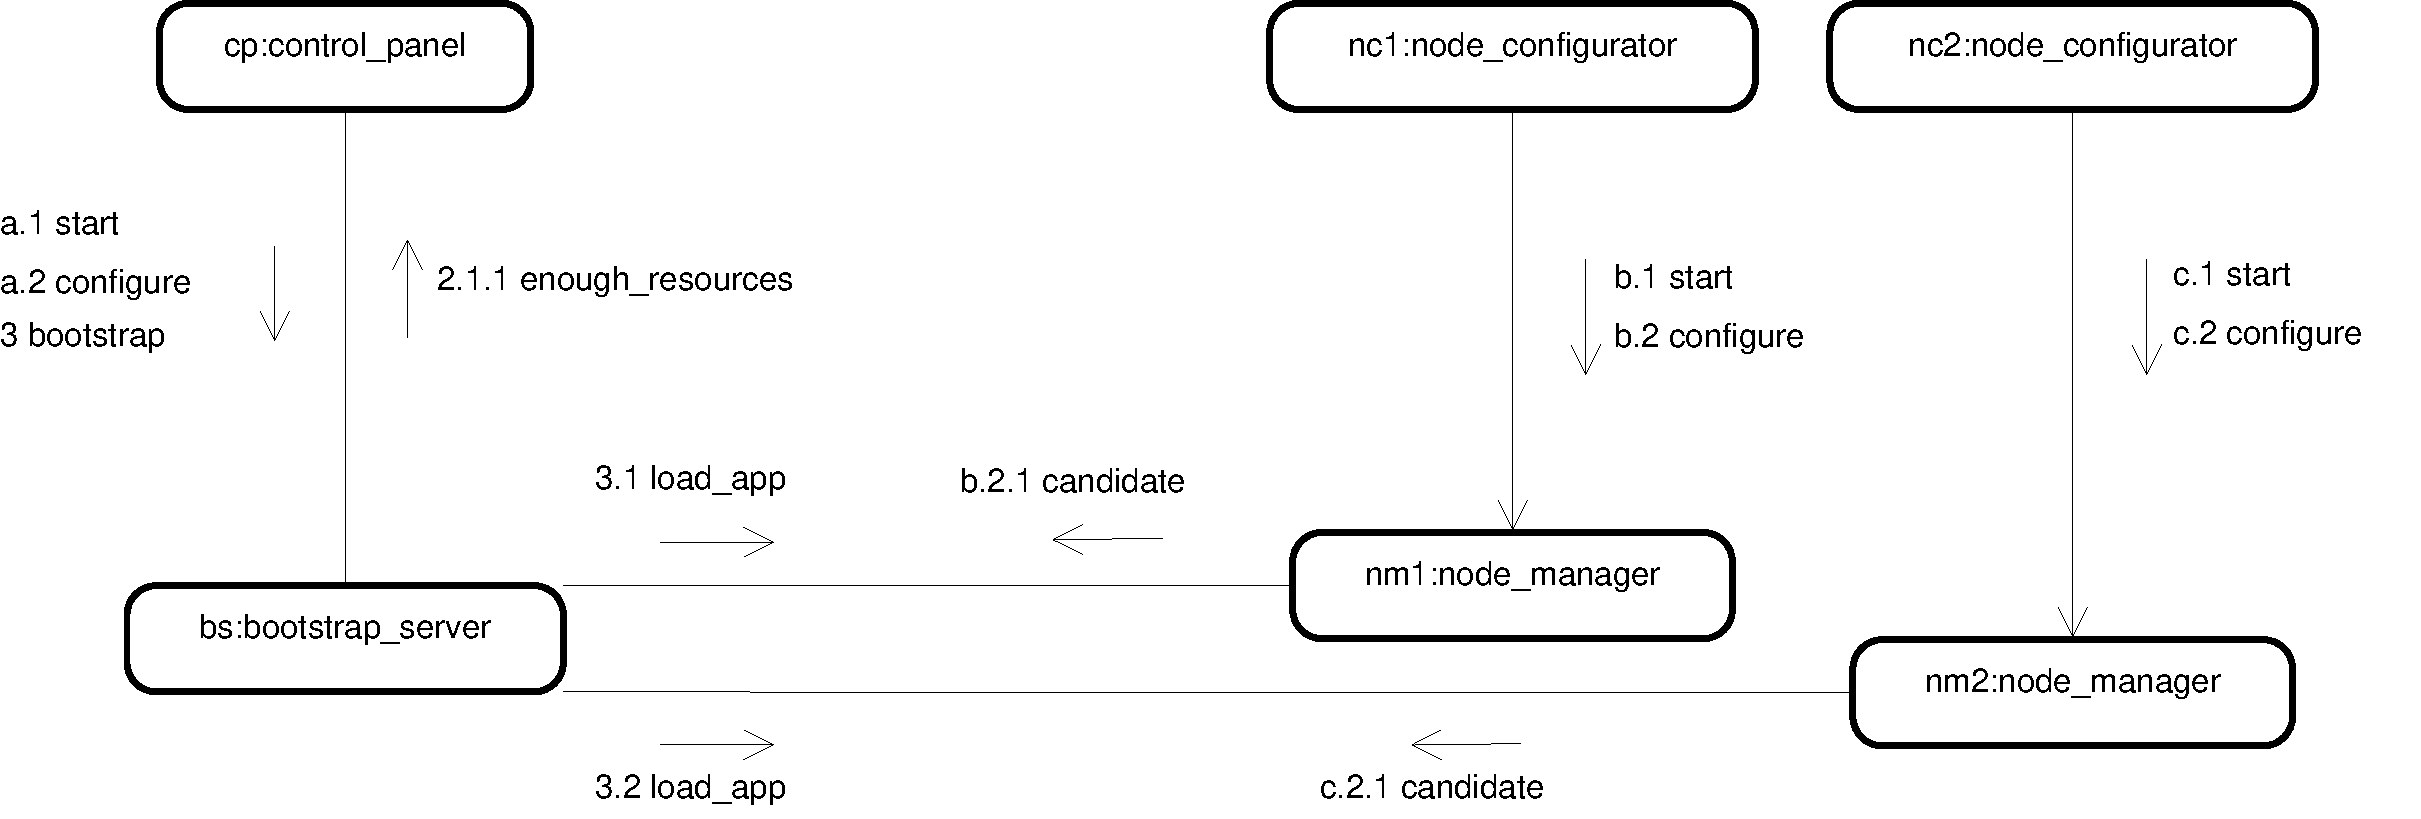
\includegraphics[height=.24\paperheight]{diagrammi/Bootstrap}
\caption{Diagramma della fase di \textit{bootstrap}}
\label{fig:bootstrap}
\end{figure}
\end{landscape}

Effettuando il \textit{parsing} dei file di configurazione, la logica di \fun{read\_config\_files} è in grado di calcolare la richiesta di risorse di simulazione necessarie, mentre \fun{node\_manager:configure}, con il metodo \fun{add\_node} comunica a \texttt{bootstrap\_server} le disponibilità di risorse di quel nodo. Una volta raggiunta la quota necessaria di risorse viene inviato il messaggio \fun{ready} a \texttt{control\_panel} che può quindi abilitare il pulsante di \textit{bootstrap}.

A questo punto l'utente può interagire con l'interfaccia grafica e causare l'invocazione del metodo \fun{bootstrap\_server:bootstrap} che provvede a inizializzare \textsl{Mnesia} e creare le tabelle vuote che verranno successivamente utilizzate dal sistema. Grazie alle informazioni di configurazione viene anche generata la tabella contenente la descrizione della pista. Successivamente il metodo \fun{bootstrap} istanzia, attraverso \fun{node\_manager:start\_app}, tutte le componenti di simulazione necessarie, nell'ordine:
\begin{enumerate}
\item \texttt{event\_dispatcher}
\item \texttt{scheduler}
\item \texttt{weather}
\item \texttt{team}
\item \texttt{car}
\end{enumerate}

Così si conclude la fase di avvio del sistema e si può passare quindi alla fase di simulazione.

\section{Dinamiche della competizione}
\subsection{Partenza}
Prima che l'utente possa dare il via alla competizione tutte le auto devono essersi registrate presso lo \texttt{scheduler} indicando come tempo di prenotazione $0$. \`E importante precisare che, in questa situazione, l'ordine in cui lo \texttt{scheduler} permette ai processi \texttt{car} di andare in esecuzione non influenza l'esito della gara: infatti alla partenza le auto sono tutte su segmenti diversi e di conseguenza non concorrono tra di loro per l'accesso ad uno stesso segmento. Ne deriva quindi che sebbene l'ordine di esecuzione alla partenza possa essere considerato casuale (dipende dall'ordine di registrazione presso lo \texttt{scheduler}, che è una componente distribuita del sistema), questo non va ad influenzare i tempi di percorrenza dei segmenti da parte delle auto e non influisce quindi con il risultato della gara.
La disposizione iniziale delle auto sulla pista avviene similmente a quanto riportato in figura~\ref{fig:startGrid}, ed è richiesto all'utente che nella zona di pista che precede la linea di arrivo vi siano almeno tre corsie.

\begin{figure}
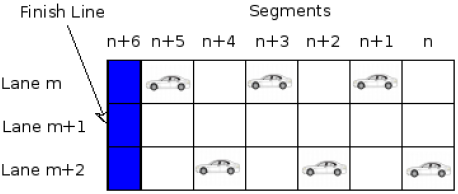
\includegraphics[width=\textwidth]{diagrammi/StartGrid}
\caption{Griglia di partenza}
\label{fig:startGrid}
\end{figure}

\subsection{Percorrenza di un segmento}
\label{sec:percorrenza}
Nel momento in cui un'auto si appresta a percorrere un segmento sono noti:
\begin{itemize}
\item corsia di ingresso,
\item velocità di ingresso,
\item tempo di ingresso,
\item conformazione e stato del segmento,
\item caratteristiche e stato dell'auto,
\item informazioni su altre auto che stanno percorrendo quel segmento.
\end{itemize}

Grazie alle informazioni sopra elencate e indicando in quale corsia il pilota vuole trovarsi all'uscita del segmento è possibile calcolare il tempo e la velocità di uscita dell'auto. Sono principalmente due i gruppi di fattori che influenzano questo calcolo: in primo luogo l'auto stessa e le caratteristiche della pista, poi la presenza di altre auto nello stesso segmento e l'interazione con esse.

Iniziando ad analizzare il primo gruppo di fattori risulta evidente che vi è una velocità massima che un'auto può mantenere in un segmento per evitare di uscire di pista, in particolare nei segmenti curvilinei la forza di attrito deve essere sufficiente a contrastare la forza centrifuga.
Visto che la forza d'attrito dipende anche dalle caratteristiche e dallo stato dell'auto, ne consegue che tale velocità massima può essere diversa per ogni auto.
Un altro vincolo alla velocità è dato dal regolamento di gara per quanto riguarda la percorrenza della \textit{pit lane}, tuttavia questo vincolo non riguarda l'intero segmento ma solo una determinata corsia e va applicato solo sulle auto che stanno per rientrare ai \textit{box} per effettuare una sosta.

I segmenti appena considerati non sono tuttavia gli unici ad avere un limite alla velocità alla quale possono essere percorsi. Basta pensare alle azioni che i piloti effettuano prima di intraprendere una curva nella realtà per capire che un segmento curvilineo impone vincoli alla velocità di percorrenza anche nei segmenti che lo precedono. \`E quindi corretto affermare che ogni segmento della pista ha un limite di velocità, sia esso diretto o indiretto.

Inoltre il numero di segmenti che impone limiti di velocità diretti può cambiare in base al fatto che il pilota voglia o meno effettuare una sosta ai \textit{box}. Di conseguenza cambieranno anche i limiti indiretti. Per questo motivo abbiamo deciso di modellare questo fatto associando ad ogni segmento due limiti di velocità, aggiornati dinamicamente nel corso della competizione: uno da rispettare nel caso in quel giro non si voglia effettuare una sosta ai box, l'altro nel caso opposto. In caso di sosta ai box è necessario infatti che la vettura mantenga, in prossimità dell'ingresso alla \textit{pitlane}, una velocità sufficientemente bassa da permettere di rallentare prima di effettuare l'ingresso nella zona sottoposta a limite di velocità dal regolamento.

La fase in cui vengono calcolati i due limiti di velocità per ogni segmento della pista è detta ``fase di preelaborazione'' e viene effettuata da ciascuna auto:
\begin{enumerate}
\item all'inizio della gara;
\item ogni volta che passa per il traguardo;
\item dopo ogni sosta ai \textit{box};
\item dopo ogni cambio delle condizioni atmosferiche.
\end{enumerate}
Il calcolo al punto 1 avviene poiché non è possibile per un'auto effettuare una mossa senza avere una tabella di preelaborazione, al punto 2 per avere una stima più accurata dei valori necessari che consideri il livello di carburante e usura pneumatici attuale e ai punti 3 e 4 poiché in corrispondenza di tali eventi può cambiare di molto l'attrito pneumatici/pista e invalidare quindi la preelaborazione precedente.

Nel calcolo dei limiti di velocità indiretti è molto importante la decelerazione massima che un'auto può raggiungere: per rendere la simulazione più verosimile abbiamo deciso di trattare in modo abbastanza dettagliato la parte fisica della competizione, facendo dipendere accelerazione e decelerazione massime sia dalle caratteristiche dell'auto che da quelle della pista.
In particolare l'accelerazione/decelerazione che un auto può erogare in un determinato segmento dipende da:
\begin{itemize}
\item potenza del motore/dei freni,
\item peso dell'auto a secco,
\item peso del pilota,
\item peso del carburante,
\item stato di usura e tipo dei pneumatici,
\item condizioni atmosferiche,
\item inclinazione della pista.
\end{itemize}

\begin{figure}
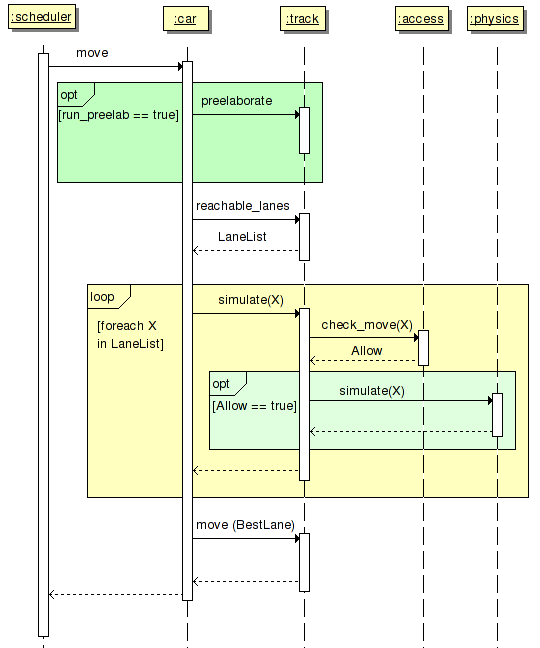
\includegraphics[width=\textwidth]{diagrammi/Simulation}
\caption{Fase di simulazione}
\label{fig:simulation}
\end{figure}

Passiamo ora a descrivere le operazioni che il processo \texttt{car} effettua nel momento in cui lo \texttt{scheduler} gli consente di eseguire una mossa.

Come si può vedere in figura~\ref{fig:simulation}, la prima operazione è l'eventuale ricalcolo della tabella di preelaborazione; successivamente viene controllato se è prevista una sosta ai \textit{box} per il giro corrente; infine si passa alla fase di simulazione vera e propria. Nella fase di simulazione \texttt{car} richiede a \texttt{track} quali sono le corsie raggiungibili nel segmento che sta per percorrere e successivamente di simulare l'esito dello spostamento per ogni corsia che l'auto può raggiungere. Questa fase, implementata da \fun{track:simulate}, può restituire diversi risultati a \texttt{car}.
\begin{itemize}
\item \texttt{race\_ended}: l'auto nella mossa precedente ha superato il traguardo nell'ultimo giro e ha quindi terminato la sua gara.
\item \texttt{fail}: l'auto non può effettuare la mossa richiesta a causa di uno dei seguenti motivi:
	\begin{itemize}
	\item il carburante è esaurito;
	\item i pneumatici sono esplosi per l'eccessiva usura;
	\item la scuderia ha ordinato il ritiro dell'auto dalla competizione;
	\item non è possibile occupare la corsia richiesta poiché il regolamento lo vieta;
	\item si sta cercando di entrare nella \textit{pit lane} senza aver segnalato la sosta;
	\item la corsia che si vuole percorrere è già occupata e la capacità di frenata non è sufficiente ad accodarsi all'auto che precede;
	\item l'auto non è in grado di mantenersi in pista a causa della velocità eccessiva.
	\end{itemize}
\item \texttt{pits}: l'auto effettuerà una sosta ai \textit{box}.
\item \texttt{Time}: il tempo in cui l'auto uscirà da quel segmento calcolato come tempo di ingresso più tempo di percorrenza.
\end{itemize}
Una volta ottenuti i risultati della simulazione, la logica di \texttt{car} decide quale sia la corsia migliore da percorrere, in particolare l'auto sceglierà la corsia la cui simulazione ritorna il valore (in ordine di priorità decrescente):
\begin{enumerate}
\item \texttt{race\_ended};
\item \texttt{pits};
\item il valore \texttt{Time} minore;
\item \texttt{fail}.
\end{enumerate}

\begin{figure}
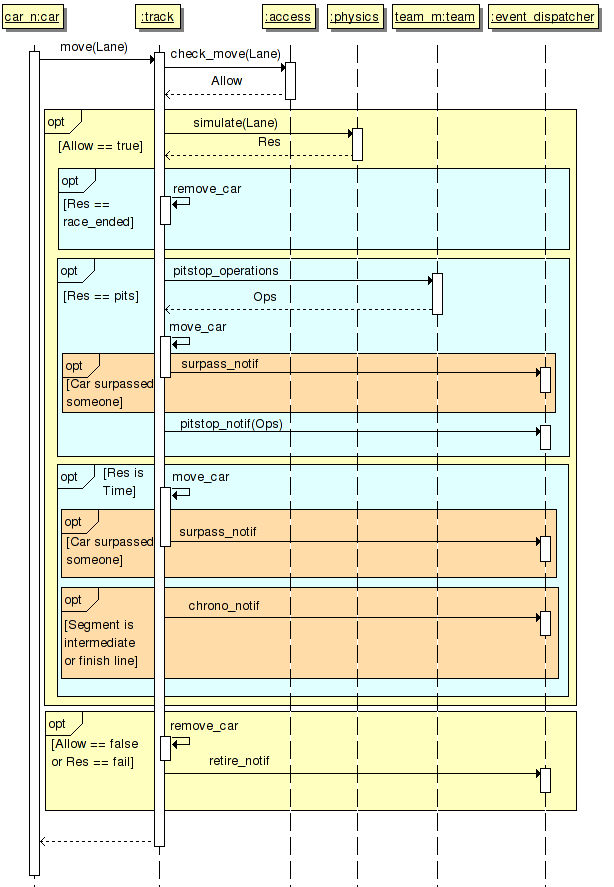
\includegraphics[width=\textwidth]{diagrammi/Move}
\caption{Fase di spostamento}
\label{fig:move}
\end{figure}

Una volta scelta la corsia migliore \texttt{car} effettua lo spostamento sulla pista grazie all'invocazione \fun{track:move} (figura~\ref{fig:move}) e resta in attesa del risultato che può essere o il tempo di uscita dal segmento che si sta percorrendo oppure \texttt{race\_ended} oppure \texttt{fail}. Nel primo caso l'auto provvederà a prenotarsi presso lo \texttt{scheduler} indicando il tempo di uscita, negli altri casi \texttt{car} non effettuerà alcuna nuova prenotazione.

La prima parte della fase di spostamento è molto simile alla fase di simulazione poiché viene controllato se la mossa è consentita o meno e viene eventualmente calcolato il tempo di uscita anche nel caso in cui si tratti di una sosta ai \textit{box}. Nella seconda parte dello spostamento vengono emesse eventuali notifiche verso \texttt{event\_dispatcher}.

Il metodo \fun{move\_car} è particolarmente importante ai fini della simulazione poiché serve a individuare eventuali sorpassi avvenuti all'interno del segmento e notificarli. Un ulteriore compito del suddetto metodo è quello di aggiornare lo stato di \texttt{track} contenuto nel \textit{database}.

Il metodo \fun{move\_car} deve anche calcolare i consumi dell'auto derivanti dall'aver percorso quel segmento.
Il consumo di carburante è pari a una quantità fissa per segmento moltiplicata per un coefficiente dipendente dall'inclinazione della pista in quel punto, mentre il consumo dei pneumatici dipende dalla curvatura del segmento, dal tipo di pneumatici usati e dalle condizioni atmosferiche.

\subsection{Intermedi cronometrici}
Gli intermedi cronometrici e il traguardo sono dei particolari segmenti aventi lunghezza nulla. Dal punto di vista di \texttt{car} sono trattati esattamente come tutti gli altri segmenti in quanto è compito di \texttt{track} nascondere le differenze ed effettuare semplificazioni dove possibile. Avendo lunghezza zero, non è necessario effettuare il calcolo del tempo di percorrenza. Infatti per questo tipo di segmenti, detti:
\begin{itemize}
\item $n+1$: l'indice di tale segmento;
\item $L_{ex_A}^{n}$: la corsia di uscita di A dal segmento $n$;
\item $L_{ex_A}^{n+1}$: la corsia di uscita di A dal segmento $n+1$;
\item $T_{en_A}^{n+1}$: il tempo di ingresso di A nel segmento $n+1$;
\item $T_{ex_A}^{n}$: il tempo di uscita di A dal segmento $n$;
\item $T_{ex_A}^{n+1}$: il tempo di uscita di A dal segmento $n+1$;
\end{itemize}
allora valgono:
\begin{itemize}
\item $L_{ex_A}^{n} = L_{ex_A}^{n+1}$: imposto dal modulo \texttt{access} poiché non è possibile cambiare corsia in un segmento di lunghezza nulla;
\item $T_{ex_A}^{n} = T_{en_A}^{n+1} = T_{ex_A}^{n+1}$: poiché il tempo impiegato a percorrere un tratto di lunghezza nulla è nullo;
\item la velocità di uscita dal segmento $n+1$ è uguale alla velocità di ingresso nel medesimo segmento;
\item non possono avvenire sorpassi all'interno di tale segmento;
\item il percorrere tale segmento non causa consumo né di carburante né di pneumatici.
\end{itemize}
Come si può notare in figura~\ref{fig:move} in corrispondenza del transito di un'auto attraverso un intermedio cronometrico viene emessa da \texttt{track} una \texttt{chrono\_notif} verso \texttt{event\_dispatcher}. Questo tipo di messaggio contiene:
\begin{itemize}
\item ID dell'auto;
\item ID dell'intermedio e numero del giro;
\item tempo di gara in cui l'auto attraversa l'intermedio;
\item velocità massima raggiunta dall'auto dopo l'intermedio precedente;
\item stato corrente di carburante e pneumatici dell'auto.
\end{itemize}

\subsection{Pit lane}
\begin{figure}
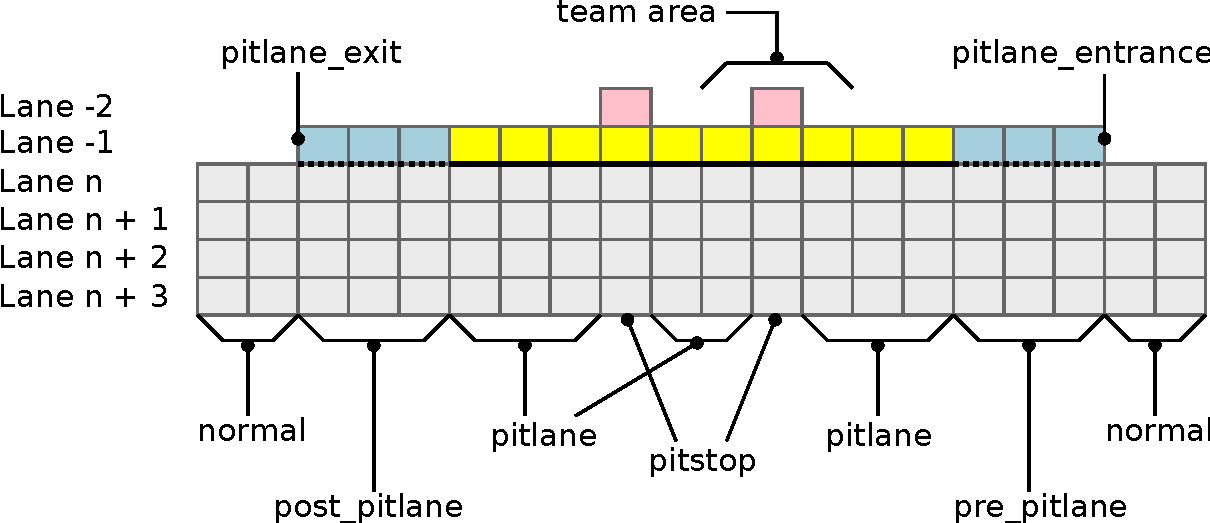
\includegraphics[width=\textwidth]{diagrammi/PitLane}
\caption{Rappresentazione della zona dei \textit{box}}
\label{fig:pitLane}
\end{figure}

La sezione di pista indicata dall'utente come zona \textit{box} (attraverso l'impostazione di \texttt{pitlane\_entrance} e \texttt{pitlane\_exit} nel file di configurazione) viene rappresentata dalla componente \texttt{track} come mostra la figura~\ref{fig:pitLane}. Le corsie con indice maggiore o uguale a $n$ sono quelle indicate dall'utente nel file di configurazione mentre le corsie $-1$ e $-2$ sono generate in modo automatico in fase di costruzione della pista.

Per ogni \texttt{team} che partecipa alla simulazione viene riservata una zona \textit{box} diversa (indicata in figura come \textit{team area}) formata da due segmenti di tipo \texttt{pitlane} ed uno di tipo \texttt{pitstop}. Per poter effettuare il rifornimento un'auto deve trovarsi nella corsia di indice $-2$ del segmento \texttt{pitstop} associato alla sua scuderia.

I segmenti di tipo \texttt{pre\_pitlane}, \texttt{post\_pitlane}, \texttt{pitlane} e \texttt{pitstop} sono soggetti a regole di percorrenza aggiuntive definite nel modulo \texttt{access}.
\begin{itemize}
\item \texttt{pre\_pitlane}: non è possibile effettuare uno spostamento dalla corsia $-1$ verso la corsia $n$.
\item \texttt{post\_pitlane}: non è possibile effettuare uno spostamento dalla corsia $-1$ verso la corsia $n$ e viceversa. In particolare lo spostamento dalla corsia $-1$ verso la corsia $n$ è permesso solo dopo la fine del tratto denominato \textit{post pitlane} per evitare che le auto in uscita dalla corsia proveniente dai \textit{box} intralcino le auto sulle altre corsie che arrivano probabilmente con una velocità maggiore.
\item \texttt{pitlane}: non è possibile effettuare uno spostamento dalla corsia $-1$ verso la corsia $n$ e viceversa.
\item \texttt{pitstop}: non è possibile effettuare uno spostamento dalla corsia $-1$ verso la corsia $n$ e viceversa; inoltre un'auto non può accedere alla corsia $-2$ dei segmenti \texttt{pitstop} appartenenti ad altre scuderie.
\end{itemize}

Il regolamento delle gare di Formula Uno impone un limite di velocità nella corsia dei \textit{box}, nel caso della simulazione questo limite è applicato nelle corsie di indice $-1$ e $-2$ dei segmenti di tipo \texttt{pitlane} e \texttt{pitstop} ed è imposto alle auto nel calcolo della velocità massima eseguito in fase di preelaborazione, come precedentemente descritto.
La corsia aggiuntiva nei segmenti di tipo \texttt{pre\_pitlane} e \texttt{post\_pitlane} serve a rappresentare rispettivamente la corsia di decelerazione e la corsia di accelerazione e non sono quindi soggette a particolari limiti di velocità imposti dal regolamento.

\subsection{Rifornimento}
\label{sec:rifornimento}
Per poter effettuare le operazioni di rifornimento e cambio pneumatici un'auto deve trovarsi a percorrere il segmento \texttt{pitstop} associato alla sua scuderia nella corsia di indice $-2$. Quando \texttt{car} effettua uno spostamento in tale posizione è la componente \texttt{track} che si incarica di effettuare la chiamata alla componente \texttt{team} associata all'auto per richiedere quali operazioni siano da effettuare sull'auto durante la sosta. \texttt{track} invia quindi le informazioni sulla quantità residua di carburante e sull'usura dei pneumatici dell'auto al \texttt{team}, il quale risponde con un messaggio indicante la quantità di carburante da aggiungere e quale tipo di pneumatici montare in caso di cambio gomme.

Le componenti \texttt{team} sono in grado di calcolare questi valori sulla base dei dati ottenuti tramite \texttt{event\_dispatcher} e derivanti dalle \texttt{crono\_notif}. Grazie a questo meccanismo \texttt{team} riesce a calcolare il consumo di carburante e gomme medio sul giro per ogni auto e ad adottare quindi una strategia di rifornimento ragionevole.
Il tempo necessario ad effettuare le operazioni è calcolato da \texttt{track} in base alle operazioni da effettuare.

Visto che ogni scuderia può rifornire una sola auto alla volta il tempo di uscita dell'auto A è calcolato come segue:
\[ T_{ex_A} = \max \left\{ T_{en_A}, T_{ex_B} \right\} + T_{ops} \]
dove B è l'auto accodata nello stesso segmento e in corsia $-2$ con tempo di uscita maggiore (ovvero l'auto che eventualmente precede A nella sosta ai \textit{box}) e $T_{ops}$ è il tempo necessario ad effettuare le operazioni di rifornimento.

\begin{figure}
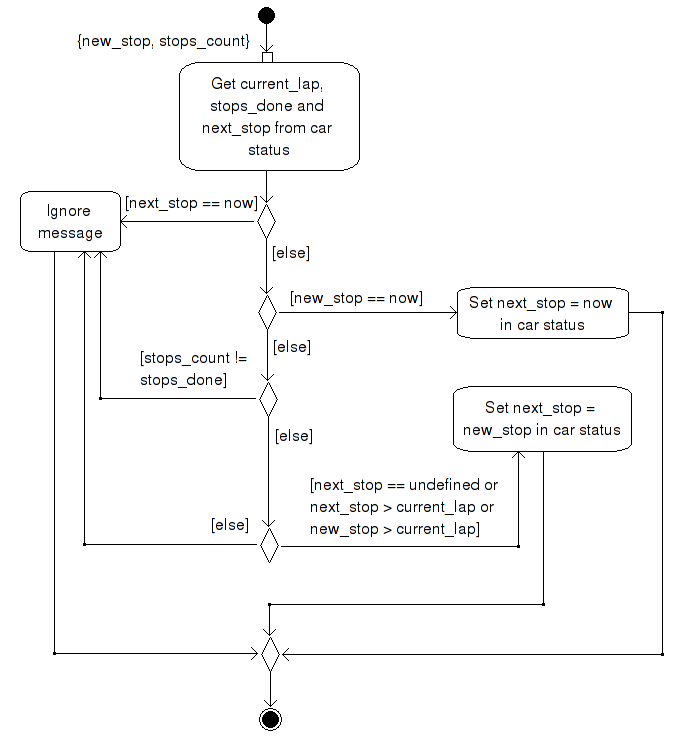
\includegraphics[width=\textwidth]{diagrammi/NextPitstop}
\caption{Algoritmo di \fun{car:set\_next\_pitstop}}
\label{fig:nextPitstop}
\end{figure}

Un'auto si reca ai \textit{box} in risposta a due eventi distinti:
\begin{itemize}
\item su richiesta dell'utente e con effetto immediato,
\item su richiesta di \texttt{team}, in base ai dati ottenuti nel corso della competizione, indicando il giro a cui l'auto deve recarsi ai \textit{box}.
\end{itemize}

Il primo tipo di richiesta arriva direttamente dalla componente \texttt{team\_monitor}, mentre il secondo tipo arriva da \texttt{team} che comunica con l'auto attraverso l'invio di un messaggio di tipo \texttt{next\_pitstop} in modo asincrono per evitare possibili situazioni di \textit{deadlock}. Il fatto che il messaggio sia asincrono introduce il problema relativo alla freschezza delle informazioni che il messaggio veicola. Supponiamo infatti di avere una conformazione della pista tale per cui appena prima del segmento \texttt{pitstop} di una scuderia vi sia un segmento di tipo \texttt{intermediate} e supponiamo anche che l'auto A di tale scuderia stia percorrendo la \textit{pit lane} per effettuare una sosta.
\`E possibile che si verifichi la seguente sequenza di eventi:
\begin{enumerate}
\item A percorre il segmento \texttt{intermediate} e viene inviata una \texttt{chrono\_notif} a \texttt{event\_dispatcher};
\item A percorre il segmento successivo ed effettua la sosta ai \textit{box};
\item la \texttt{chrono\_notif} arriva alla scuderia di A che, in base ai dati ricevuti sullo stato dell'auto (ormai obsoleti a causa del rifornimento), decide, per esempio, di posticipare al giro successivo la sosta ai \textit{box};
\item A riceve il messaggio e obbedisce alla scuderia, rientrando nuovamente ai \textit{box} nel giro successivo ed effettuando molto probabilmente una sosta inutile.
\end{enumerate}

La soluzione che abbiamo adottato per evitare questo genere di incongruenze prevede che \texttt{car} e \texttt{team} mantengano un contatore delle soste effettuate dall'auto fino a quel momento e che \texttt{team} nel messaggio \fun{next\_pitstop} inserisca anche il valore di tale contatore. Di conseguenza, nel momento in cui viene ricevuto il messaggio, l'auto può verificare la freschezza delle informazioni in esso contenute ed eventualmente ignorarlo. I messaggi provenienti dall'utente ovviamente non necessitano di tale contatore poiché sono considerati dall'auto sempre corretti.

Lato \texttt{car}, l'algoritmo che gestisce l'arrivo di messaggi \fun{next\_pitstop} è quello rappresentato in figura~\ref{fig:nextPitstop}. Il parametro \fun{new\_stop} presente nel messaggio \fun{next\_pitstop} può assumere il valore \fun{now} nel caso in cui la sosta sia imposta dall'utente oppure può essere l'indice del giro in cui effettuare il pitstop successivo se la sosta è richiesta dalla logica di \texttt{team}. Come si può notare dalla figura, viene data priorità maggiore alle decisioni dell'utente ignorando i messaggi dei \texttt{team} che potrebbero interferire. Nello stato interno dell'auto, il campo \fun{next\_stop} può assumere i valori \fun{now}, un intero positivo oppure \fun{undefined}. In particolare il valore \fun{undefined} serve ad indicare che non sono state ancora previste soste oppure che l'auto ha appena effettuato un rifornimento e non ha ancora ottenuto direttive dai \texttt{team} o dall'utente.

\subsection{Arrivo}
Un'auto termina la competizione nel momento in cui va a percorrere il segmento successivo al traguardo nell'ultimo giro di gara oppure se si ritira, come descritto in~\ref{sec:percorrenza}. Come si può notare in figura~\ref{fig:move}, nel momento in cui un'auto esce dalla competizione viene invocato il metodo \fun{track:remove\_car} e successivamente il processo termina la propria esecuzione.

Tale metodo serve anche a mantenere aggiornato il contatore delle auto ancora in gara interno alla componente \texttt{track}. Nel momento in cui questo contatore raggiunge il valore zero allora la gara è terminata e \texttt{track} può notificare questo evento al resto del sistema tramite \texttt{event\_dispatcher}.

In questo modo le componenti del sistema non più necessarie possono terminare la propria esecuzione, mentre le componenti grafiche possono disabilitare le funzionalità non più disponibili ma restare comunque attive per permettere all'utente di consultare i dati relativi alla simulazione.

\begin{landscape}
\begin{figure}
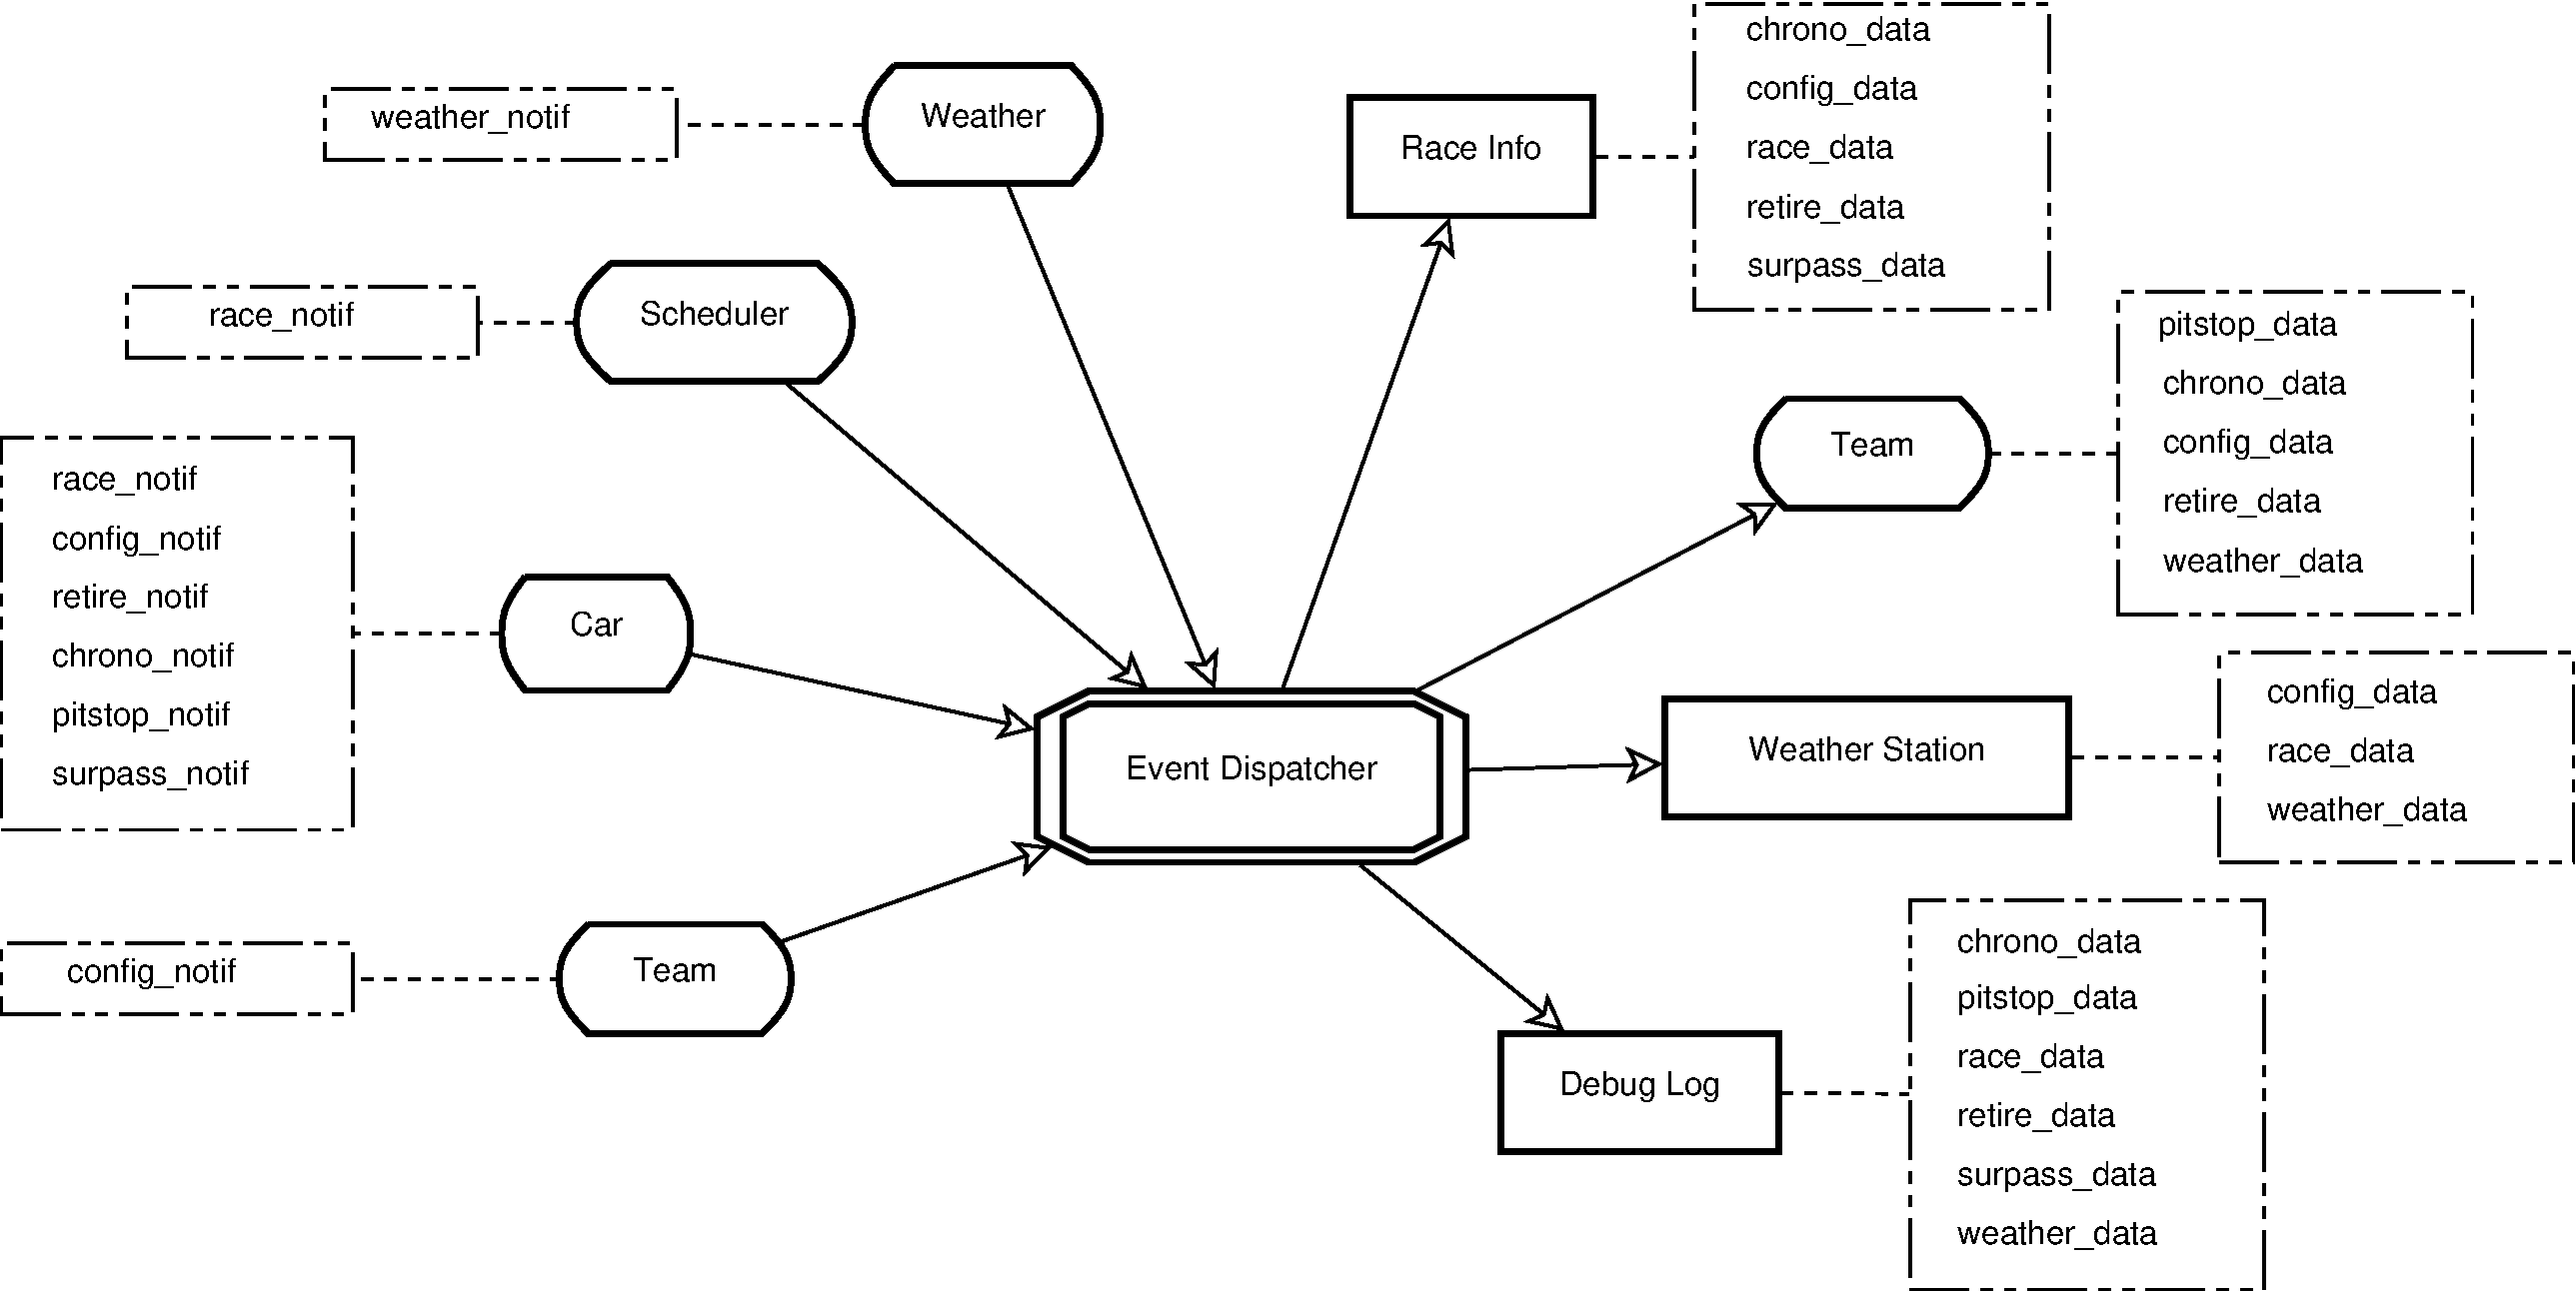
\includegraphics[width=0.75\paperheight]{diagrammi/NotifFlow}
\caption{Diffusione delle notifiche tramite \texttt{event\_dispatcher}}
\label{fig:notifFlow}
\end{figure}
\end{landscape}

\section{Event Dispatcher}
\label{sec:event_dispatcher}
In figura~\ref{fig:notifFlow}, sulla sinistra si possono vedere quali sono i tipi di notifica presenti nel sistema e da che componenti sono inviati, mentre sulla destra sono rappresentate le componenti che ricevono i dati, eventualmente rielaborati, derivanti dalle notifiche.

Un compito molto importante di \texttt{event\_dispatcher} è quello di mantenere l'ordine delle notifiche rispetto ogni destinazione, non è quindi possibile affidarsi a comunicazioni asincrone.
I messaggi in ingresso e in uscita da \texttt{event\_dispatcher} verso le altre componenti del sistema sono quindi veicolati da chiamate sincrone, tuttavia, al suo interno \texttt{event\_dispatcher} è composto da più processi che comunicano tra di loro in modo asincrono, mantenendo comunque invariato l'ordine delle notifiche.
Questo è possibile poiché l'ordine di messaggi asincroni tra processi sullo stesso nodo è garantito dal linguaggio.

\begin{figure}
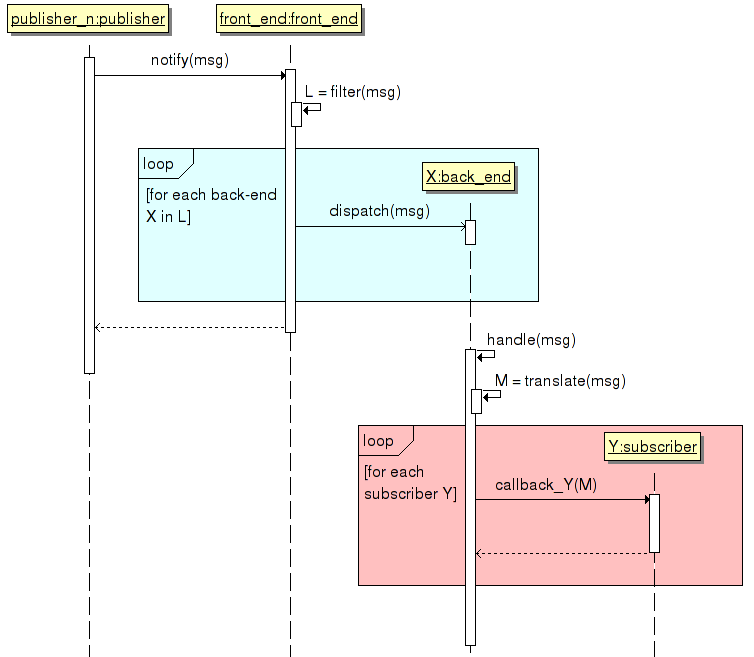
\includegraphics[width=\textwidth]{diagrammi/Dispatcher}
\caption{Funzionamento interno di \texttt{event\_dispatcher}}
\label{fig:dispatcher}
\end{figure}

Come si può vedere in figura~\ref{fig:dispatcher}, \texttt{event\_dispatcher} è composto di un processo detto \textit{front-end} che ha il compito di ricevere ogni notifica in ingresso e inoltrarla ai \textit{back-ends} interessati in modo asincrono. Oltre a ciò, il \textit{front-end} deve anche ricevere le richieste di \textit{subscription} e registrare quindi i processi richiedenti presso il corretto \textit{back-end}. Al ricevimento di una notifica un \textit{back-end} provvede ad una eventuale rielaborazione dei dati in essa contenuti per poi inviare il risultato di tale computo ai processi presenti nella sua lista di \textit{subscribers}.

Poiché è stato previsto che una GUI possa registrarsi a simulazione iniziata è necessario che i \textit{back-ends} mantengano uno stato interno in modo da poter inviare al processo che si registra un'immagine parziale dello stato della competizione fino al momento della \textit{subscription}. Successivamente, al processo richiedente verranno inviate solo le informazioni contenenti i cambiamenti relativi allo stato della competizione e non lo stato stesso in modo da ridurre la quantità di dati inviati. In questo modo non vengono inviati dati ridondanti.


\chapter{Correttezza}
\section{Avvio del sistema}
L'avvio del sistema è coordinato da \texttt{bootstrap\_server} che stabilisce l'ordine di avvio delle componenti del sistema (come descritto nella sezione~\ref{sec:avvio}) e controlla che l'avvio delle stesse avvenga in modo corretto.

\texttt{event\_dispatcher} è la prima componente ad essere avviata in modo da permettere l'invio di \fun{config\_notif} da parte delle componenti del sistema durante la loro fase di avvio.

Successivamente viene avviato lo \texttt{scheduler} di modo che i processi \texttt{weather} e \texttt{car} possano prenotarsi per l'esecuzione e l'accesso a \texttt{track}. In questo modo ogni componente del sistema dispone delle informazioni e delle altre componenti necessarie affinché il proprio avvio avvenga correttamente.

Nel caso in cui qualcuna delle componenti del sistema non riuscisse ad avviarsi questo sarebbe rilevato da \texttt{bootstrap\_server} e comunicato all'utente. Di conseguenza, se l'esecuzione del metodo \fun{bootstrap\_server:bootstrap} termina senza errori vuol dire che la simulazione è pronta ad essere avviata.

Una possibile situazione di errore si può avere nel caso in cui vengano istanziati due nodi \Erlang{} con lo stesso nome. Ciò tuttavia è estremamente improbabile poiché la parte del nome che viene generata casualmente da \texttt{node\_configurator} è una stringa di 8 cifre esadecimali. Nel caso in cui si verifichi una situazione del genere non è possibile riparare all'errore ed è quindi necessario riavviare il sistema.

\section{Accesso alla pista}
L'accesso alla componente \texttt{track} è disciplinato dallo \texttt{scheduler}; gli unici processi che vi possono accedere sono \texttt{car} e \texttt{weather}. Ogniqualvolta \texttt{car} o \texttt{weather} necessitino dell'accesso alla risorsa \texttt{track}, essi effettuano la procedura di prenotazione presso lo \texttt{scheduler} a cui è delegato il compito di gestire il protocollo di accesso a \texttt{track}.

La componente \texttt{scheduler} utilizza una politica \textit{FIFO within priorities} per gestire la coda dei processi prenotati, assegnando priorità maggiore ai processi che indicano un tempo minore in fase di prenotazione. Viene eletto un solo processo alla volta (la testa della coda) per l'accesso a \texttt{track} e non è permesso l'accesso ad altri processi. Questo finché il processo che sta utilizzando \texttt{track} non notifica allo \texttt{scheduler} di non aver più bisogno della risorsa.

Lo \texttt{scheduler} garantisce quindi un accesso sequenziale a \texttt{track} e assicura che la pista si trovi sempre in uno stato consistente.

\section{Tempo di percorrenza}
Il tempo che un'auto impiega a percorrere la pista è la somma del tempo impiegato a percorrere i singoli segmenti ed è calcolato algoritmicamente dalla componente \texttt{track}. Risulta quindi evidente che il sistema su cui sta eseguendo l'applicazione non influisce minimamente sui tempi di percorrenza delle auto, tanto meno influisce l'orologio di sistema. Il tempo di percorrenza di un segmento da parte di un'auto è influenzato dagli altri partecipanti solo qualora le traiettorie delle auto si intersechino.

Non è possibile che avvenga il fenomeno dello ``scavalcamento'' tra auto, per convincersi di ciò basta analizzare attentamente l'algoritmo che gestisce il calcolo del tempo di percorrenza di un segmento e l'eventuale interazione tra le auto.

\begin{figure}
\begin{center}
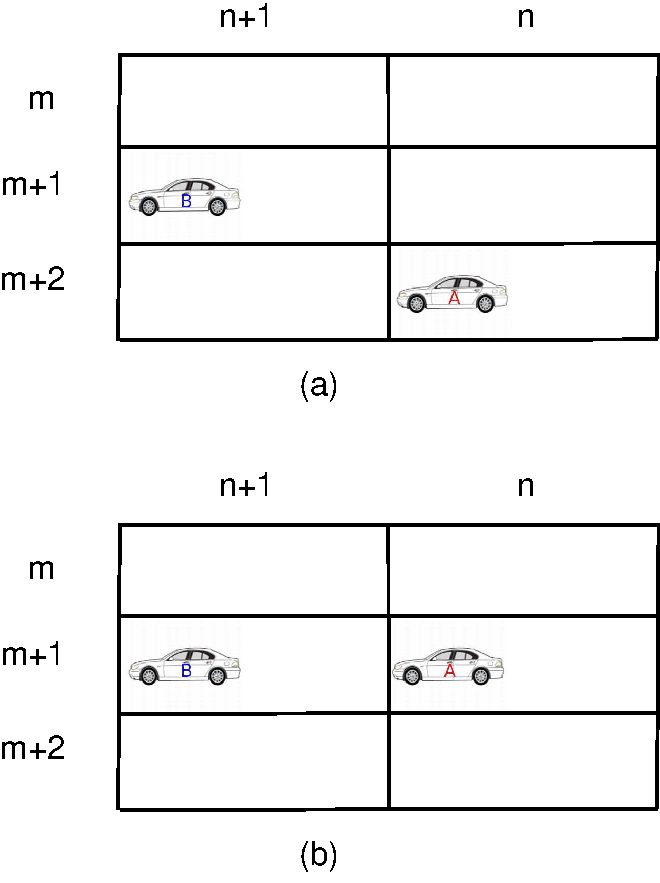
\includegraphics[width=0.5\textwidth]{diagrammi/Surpass}
\caption{Interazione tra auto nello stesso segmento}
\label{fig:surpass}
\end{center}
\end{figure}
La figura~\ref{fig:surpass} rappresenta le situazioni che si possono creare nel momento in cui un'auto percorre un segmento di pista in cui è presente un altra auto.

Individuare le auto sorpassate a seguito della mossa che un'auto (chiamiamola A) sta effettuando è semplice: detto $T_{en_X}$ il tempo di ingresso di un'auto X nel segmento e $T_{ex_X}$ il suo tempo di uscita, l'insieme delle auto $\mathcal{S}$ sorpassate da A in quel segmento sarà:
\[ \mathcal{S} = \{ X \mid T_{en_X} \leq T_{en_A} \;\wedge\; T_{ex_X} > T_{ex_A}\} \]

Nel momento in cui l'auto A effettua il suo turno sono noti:
\begin{itemize}
\item $T_{en_B}^{n+1}$: il tempo di ingresso di B nel segmento $n+1$,
\item $T_{ex_B}^{n+1}$: il tempo di uscita di B dal segmento $n+1$,
\item $L_{en_B}^{n+1}$: la corsia di ingresso di B nel segmento $n+1$,
\item $L_{ex_B}^{n+1}$: la corsia di uscita di B dal segmento $n+1$,
\item $T_{en_A}^{n+1}$: il tempo di ingresso di A nel segmento $n+1$,
\item $L_{en_A}^{n+1}$: la corsia di ingresso di A nel segmento $n+1$,
\item $L_{ex_A}^{n+1}$: la corsia di uscita di A dal segmento $n+1$ (scelta dall'auto quindi si può considerare fissata).
\end{itemize}
Obiettivo dell'algoritmo è quindi il calcolo di $T_{ex_A}^{n+1}$. Sia $T_{lc}$ il tempo che un'auto impiega a spostarsi da una corsia ad una adiacente: esso è considerato fisso ed uguale per tutte le auto e ogni auto può spostarsi di una sola corsia per ogni segmento.
Come precondizione si ha inoltre che $T_{en_B}^{n+1} \leq T_{en_A}^{n+1}$ poiché B si è spostata in quel segmento prima di A, e che $T_{en_A}^{n+1} \leq T_{ex_B}^{n+1}$ altrimenti lo \texttt{scheduler} avrebbe eletto B per l'esecuzione al posto di A.

Per poter calcolare il tempo di uscita di A dal segmento $n+1$ è necessario prima valutare se B interferisce con la mossa di A.
Considerando lo scenario~(a) di figura~\ref{fig:surpass} possiamo distinguere due casi:
\begin{enumerate}
\item $L_{ex_A}^{n+1} = m+2$: non vi è alcuna interferenza da parte di B poiché la corsia $m+2$ è libera.
\item $L_{ex_A}^{n+1} = m+1$:
        \begin{enumerate}
        \item $L_{en_B}^{n+1} = m+2$: A sta seguendo esattamente la stessa traiettoria che ha seguito B per percorrere il segmento $n+1$ ed è quindi corretto che l'auto A si accodi a B e non possa superarla.
        \item $L_{en_B}^{n+1}  = m+1$: A cerca di inserirsi davanti a B tagliandole la strada; tuttavia, visto che $T_{en_B}^{n+1} \leq T_{en_A}^{n+1}$, vale anche che $T_{en_B}^{n+1} \leq T_{en_A}^{n+1} + T_{lc}$ e non è quindi possibile che A si posizioni davanti a B.
        \item $L_{en_B}^{n+1} = m$: A e B si spostano entrambe sulla stessa corsia $m+1$ provenendo da corsie differenti ma visto che $T_{en_B}^{n+1} \leq T_{en_A}^{n+1}$ allora vale anche $T_{en_B}^{n+1} + T_{lc} \leq T_{en_A}^{n+1} + T_{lc}$ e di conseguenza A può solo accodarsi a B.
        \end{enumerate}
\end{enumerate}

Per quanto riguarda lo scenario~(b) di figura~\ref{fig:surpass} vi sono due casi:
\begin{enumerate}
\item $L_{ex_A}^{n+1} = m+2$ oppure $L_{ex_A}^{n+1} = m$: non vi è alcuna interferenza da parte di B poiché le corsie sono libere.
\item $L_{ex_A}^{n+1} = m+1$:
        \begin{enumerate}
        \item $L_{en_B}^{n+1} = m+1$: A si accoda a B (vedi caso 1.a dello scenario (a)).
        \item $L_{en_B}^{n+1} = m+2$ oppure $L_{en_B}^{n+1} = m$: A cerca di inserirsi davanti a B prima che questa occupi la corsia $m+1$ e se $T_{en_B}^{n+1} + T_{lc} < T_{en_A}^{n+1}$ vuol dire che A deve accodarsi a B, altrimenti è A ed essere in testa e non viene quindi influenzata dalla presenza di B.
        \end{enumerate}
\end{enumerate}

Nei casi in cui non vi è interferenza da parte di B nella mossa di A, $T_{ex_A}^{n+1}$ viene calcolato solo sulla base delle caratteristiche dell'auto e della pista.
Nei casi in cui A deve accodarsi a B viene aggiunto il vincolo che $T_{ex_A}^{n+1} > T_{ex_B}^{n+1}$ e calcolata la velocità di uscita di conseguenza.

La procedura di sosta ai \textit{box} differisce nel calcolo del tempo di percorrenza rispetto agli altri segmenti, tuttavia si integra perfettamente nell'algoritmo citato in precedenza in quanto l'auto rimane comunque soggetta ai meccanismi di uno spostamento generico sulla pista quali il cambio corsia e il sorpasso.


L'ultima considerazione riguarda l'influenza che il fattore di \textit{simulation speed} può avere sulla competizione, ed anche in questo caso è facile convincersi che la velocità con la quale viene eseguita la simulazione non influenza in alcun modo i tempi di percorrenza delle auto. Il fattore di \textit{simulation speed} infatti viene implementato aumentando o riducendo il periodo di pausa che lo \texttt{scheduler} fa trascorrere tra il rilascio della componente \texttt{track} da parte di un processo e la concessione di tale risorsa ad un altro. Tale pausa è introdotta artificialmente per rallentare l'evolvere della simulazione e renderla quindi fruibile dall'utente.

\section{Non determinismo}
Abbiamo limitato il non determinismo a livello di simulazione alle sole situazioni in cui esso sia desiderabile. L'unico caso in cui l'ordine di esecuzione può infatti influire sul risultato della simulazione è quello in cui anche nella realtà non si riesce a prevedere in modo certo l'esito dell'interazione tra due auto.

\begin{figure}
\begin{center}
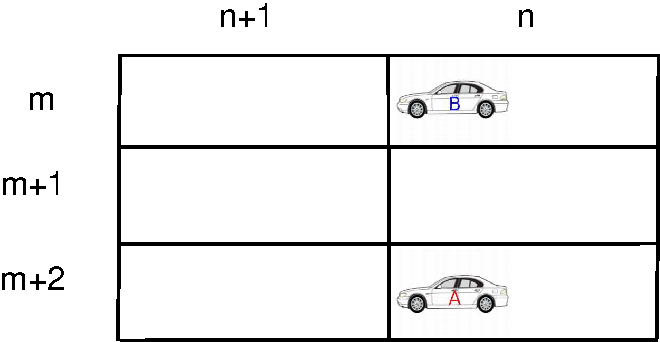
\includegraphics[width=0.6\textwidth]{diagrammi/NonDet}
\caption{Esemplificazione di una situazione di non determinismo}
\label{fig:nonDet}
\end{center}
\end{figure}

Consideriamo lo scenario riportato in figura~\ref{fig:nonDet}, e assumiamo che:
\begin{itemize}
\item le auto e i piloti abbiano caratteristiche identiche;
\item $T_{en_A}^{n+1} = T_{en_B}^{n+1}$: le auto abbiano tempi di ingresso uguali;
\item $V_{en_A}^{n+1} = V_{en_B}^{n+1}$: le auto abbiano velocità di ingresso uguali.
\end{itemize}

Sotto queste ipotesi non vi sono problemi di interazione tra le auto finché $L_{ex_A}^{n+1} \neq L_{ex_B}^{n+1}$ poiché, avendo traiettorie che non si intersecano, i tempi di percorrenza dell'una non sono influenzabili in alcun modo dall'altra.

Se tuttavia si presentasse il caso in cui $L_{ex_A}^{n+1} = L_{ex_B}^{n+1}$ allora vi sarebbe del non determinismo, in quanto il tempo di percorrenza del segmento senza considerare l'influenza delle altre auto sarebbe il medesimo, ma le due auto si troverebbero allora a collidere in uscita dal segmento. La prima auto ad eseguire sarà quindi anche la prima auto ad uscire dal segmento e di conseguenza, per quanto visto in~\ref{sec:percorrenza}, la seconda auto si dovrà accodare alla prima, facendo registrare un tempo di uscita dal segmento leggermente maggiore.

C'è da dire che il verificarsi di tale situazione è altamente improbabile e non è quindi possibile cogliere questo comportamento in una generica simulazione ma bisogna invece creare una situazione \textit{ad-hoc} per ottenere dei test ripetibili e poter apprezzare la presenza del non determinismo.

\section{Deadlocks}
Durante la fase di progettazione del sistema abbiamo posto particolare attenzione alla prevenzione di situazioni di \textit{deadlock}. In particolare ci siamo resi conto che il flusso di notifiche presente nel sistema, se non trattato in modo attento poteva facilmente essere causa di situazioni di stallo.

Come si può notare in figura~\ref{fig:notifFlow}, per esempio, la componente \texttt{team} compare sia come mittente che come destinatario e se il percorso della notifica fosse totalmente sincrono si avrebbe una situazione di \textit{deadlock} dovuta al ciclo \texttt{team} $\rightarrow$ \texttt{event\_dispatcher} $\rightarrow$ \texttt{team}.

Abbiamo quindi deciso di intervenire in modo strutturale sulla componente maggiormente coinvolta nel flusso di notifiche: \texttt{event\_dispatcher}. Come descritto in~\ref{sec:event_dispatcher}, \texttt{event\_dispatcher} al suo interno usa comunicazioni asincrone appunto per evitare possibili \textit{deadlocks}, intervenendo sulla condizione di attesa circolare. In questo modo, una volta che un processo mittente ha depositato la sua notifica presso \texttt{event\_dispatcher}, non deve bloccarsi in attesa dei processi destinatari ma può continuare la sua esecuzione.

Questa soluzione ci assicura l'assenza di \textit{deadlocks} causati dalle notifiche, poiché la propagazione di queste ultime coinvolge \texttt{event\_dispatcher} che, grazie alla sua struttura interna, evita il formarsi di cicli.

\section{Realismo}
\subsection*{Fisico}
Al fine di ottenere un buon livello di realismo della simulazione da un punto di vista fisico, abbiamo deciso di far dipendere le \textit{performance} dell'auto da diversi fattori modellando i fenomeni fisici coinvolti nel miglior modo possibile, con particolare attenzione alla decelerazione.

Nella seguente tabella vengono riportati i valori utilizzati nel modello fisico della simulazione e da quali parametri di configurazione tali valori dipendono.

\begin{center}
\begin{tabular}{|l|l|}
\hline
\textbf{Valore} & \textbf{Ricavato da} \\
\hline
\multirow{5}{*}{Velocità massima in curva} & Raggio di curvatura\\
& Inclinazione del tratto\\
& Condizioni atmosferiche\\
& Tipo di pneumatici\\
& Usura dei pneumatici\\
\hline
\multirow{8}{*}{Accelerazione/Decelerazione massima} & Potenza del motore/dei freni\\
& Peso dell'auto\\
& Peso del carburante\\
& Peso del pilota\\
& Inclinazione del tratto\\
& Condizioni atmosferiche\\
& Tipo di pneumatici\\
& Usura dei pneumatici\\
\hline
\multirow{3}{*}{Consumo dei pneumatici} & Raggio di curvatura\\
& Tipo di pneumatici\\
& Condizioni atmosferiche\\
\hline
Consumo di carburante & Inclinazione del tratto\\
\hline
\end{tabular}
\end{center}

Considerando la fase di decelerazione che un'auto deve generalmente intraprendere prima di entrare in curva o prima di accedere alla \textit{pit lane}, è stato necessario introdurre nelle meccaniche di simulazione il calcolo della tabella di preelaborazione. Questo principalmente per evitare che le auto arrivassero all'entrata della curva e, non avendo il tempo di frenare, uscissero di pista sistematicamente.

\subsection*{Dinamiche di gara}
Per quanto riguarda il realismo nelle dinamiche di gara, abbiamo considerato la possibilità per un'auto di ritirarsi dalla competizione a seguito di:
\begin{itemize}
\item uscita di pista per velocità troppo elevata;
\item uscita di pista per evitare incidenti qualora l'auto non riesca a frenare in tempo per evitare gli altri concorrenti;
\item esplosione pneumatici a causa di un'eccessiva usura;
\item esaurimento del carburante;
\item potenza del motore insufficiente a percorrere il tratto.
\end{itemize}

Si è cercato poi di descrivere l'interazione tra le auto in uno stesso segmento in modo preciso, per poter distinguere le condizioni di sorpasso e quelle di accodamento anche in base alla traiettoria di un'auto. Limitare il cambio di corsia ad uno solo per segmento è stato utile per avere un maggior controllo sull'algoritmo di percorrenza di un segmento e sull'aderenza della simulazione alla realtà.


\appendix


\chapter{File di configurazione}
\section*{Team e Car}
Le impostazioni delle scuderie, delle auto e dei piloti sono contenuti in uno stesso file di configurazione.

\begin{lstlisting}
[
        {team_name, "McLaren"},
        {brake, 34000},
        {power, 25000},
        {weight, 650},
        {cars, [
                [{id, 2},
                {name, "Lewis Hamilton"},
                {skill, 6},
                {weight, 68},
                {fuel, 70},
                {tyres, slick}],
                [{id, 6},
                {name, "Heikki Kovalainen"},
                {skill, 4},
                {weight, 62},
                {fuel, 80},
                {tyres, slick}]
                ]}
].
\end{lstlisting}

I parametri di configurazione sono descritti in \Erlang{} per risparmiare tempo sfruttando le funzioni di \textit{parsing} offerte dal linguaggio. Si tratta di una lista di coppie chiave-valore la cui semantica è spiegata nella seguente tabella:

\begin{center}
\begin{tabular}{|p{0.15\textwidth}|p{0.75\textwidth}|}
\hline
\multicolumn{2}{|c|}{Scuderia e Auto}\\
\hline
\texttt{team\_name} & Nome della scuderia\\
\texttt{brake} & Potenza dei freni\\
\texttt{power} & Potenza del motore\\
\texttt{weight} & Peso dell'auto a secco\\
\texttt{cars} & Lista dei piloti e della configurazione iniziale delle auto\\
\hline
\multicolumn{2}{|c|}{Pilota e Auto}\\
\hline
\texttt{id} & Posizione nella griglia di partenza\\
\texttt{name} & Nome del pilota\\
\texttt{skill} & Abilità del pilota (intero tra 1 e 10 compresi)\\
\texttt{weight} & Peso del pilota\\
\texttt{fuel} & Carburante presente nell'auto ad inizio gara\\
\texttt{tyres} & Tipo di gomme montate sull'auto ad inizio gara\\
\hline
\end{tabular}
\end{center}

L'unico parametro opzionale tra quelli appena elencati è \texttt{id}. Nel caso in cui nel file di configurazione esista almeno un pilota in cui il parametro \texttt{id} è omesso allora l'ordine nella griglia di partenza di tutti i concorrenti sarà generato casualmente.

\section*{Track}
Il file di configurazione di \texttt{track} contiene le informazioni riguardanti la conformazione della pista espressa in settori. La configurazione è composta da una lista di tuple, ciascuna delle quali rappresenta un settore.

Di seguito la sintassi per descrivere i tipi di settore possibili e i parametri consentiti.

\begin{itemize}
\item \verb!{straight, LENGTH, MIN_LANE, MAX_LANE, INCL, RAIN}!\\ Rettilineo
\item \verb!{right, LENGTH, RADIUS, MIN_LANE, MAX_LANE, INCL, RAIN}!\\ Curva a destra
\item \verb!{left, LENGTH, RADIUS, MIN_LANE, MAX_LANE, INCL, RAIN}!\\ Curva a sinistra
\item \verb!{finish_line}!\\ Traguardo
\item \verb!{intermediate}!\\ Intermedio cronometrico
\item \verb!{pitlane_entrance}!\\ Inizio della zona dei \textit{box}
\item \verb!{pitlane_exit}!\\ Fine della zona dei \textit{box}
\end{itemize}

\begin{tabularx}{\textwidth}{|l|X|}
\hline
\texttt{LENGTH} & Lunghezza del settore in metri, possibilmente un valore multiplo di 5\\
\hline
\texttt{RADIUS} & Raggio di curvatura in metri\\
\hline
\texttt{MIN\_LANE} & Minimo indice di corsia consentito, intero positivo\\
\hline
\texttt{MAX\_LANE} & Massimo indice di corsia consentito, intero positivo\\
\hline
\texttt{INCL} & Inclinazione della pista, deve appartenere all'intervallo $(-90^\circ, +90^\circ)$\\
\hline
\texttt{RAIN} & Condizioni atmosferiche all'inizio della gara, intero tra 0 e 10 inclusi\\
\hline
\end{tabularx}

\section*{Weather}
Questo file contiene una lista di tuple, ciascuna delle quali rappresenta le variazioni del tempo atmosferico in un istante di gara.

Le tuple sono nella forma:
\[ \{\mbox{\texttt{WHEN}},\;\: [\{\mbox{\texttt{WHERE}},\; \mbox{\texttt{RAIN}}\},\; \ldots\;\: ]\} \]
\begin{itemize}
\item \texttt{WHEN}: quando, rispetto al tempo di gara, avverrà il cambiamento. Può essere espresso in secondi oppure nel formato $\{h,m,s\}$.
\item \texttt{WHERE}: in che settore avverrà il cambiamento, l'indice si riferisce alla posizione del settore nel file di configurazione della pista.
\item \texttt{RAIN}: quantità di pioggia presente nel settore, un intero nell'intervallo $[0, 10]$.
\end{itemize}

\section*{config.hrl}
Il prototipo consente di modificare delle costanti utilizzate per la simulazione.
Queste costanti sono raggruppate nel file \texttt{include/config.hrl} e una loro modifica richiede la ricompilazione del prototipo per avere effetto.

La maggior parte delle costanti presenti in questo file agisce direttamente sul modello fisico della simulazione e sulla rappresentazione interna della pista per ottenere una simulazione a grana più o meno fine. Una delle costanti più importanti è infatti la lunghezza dei segmenti in cui viene diviso il tracciato, attualmente impostata a 5 metri.

Questi valori possono essere modificati, tuttavia tale operazione è sconsigliata poiché si potrebbe facilmente dare luogo a situazioni limite nelle quali, per esempio, nessuna auto riuscirebbe a percorrere nemmeno un tratto senza uscire di pista.

Inoltre, la validità di tali valori non viene controllata dal prototipo, di conseguenza potrebbero addirittura essere sollevate eccezioni durante i calcoli (divisione per zero, estrazione di radice quadrata di un numero negativo, e così via).


\chapter{Avvio del prototipo}
Per facilitare l'utilizzo del prototipo vengono forniti degli \textit{script} di avvio.

Si noti che le seguenti componenti possono essere presenti nel sistema in istanze multiple ed avviate anche quando la simulazione è già in corso: \texttt{race\_info}, \texttt{team\_monitor}, \texttt{weather\_station} e \texttt{debug\_log}.

\subsection*{Passo 0 -- Configurazione e compilazione}
Il comando \texttt{./configure} effettua la configurazione del prototipo in base al proprio sistema. Qualora la procedura automatica non andasse a buon fine, è possibile definire le seguenti variabili d'ambiente:
\begin{itemize}
\item \texttt{ERLC}: percorso del compilatore \Erlang{};
\item \texttt{ERLCFLAGS}: \textsl{flags} per il compilatore \Erlang{};
\item \texttt{ERL}: percorso dell'interprete \Erlang{};
\item \texttt{PYTHON}: percorso dell'interprete \Python{};
\item \texttt{PYTHONPATH}: eventuali percorsi addizionali in cui cercare i moduli \Python{};
\item \texttt{PYRCC}: percorso dell'eseguibile \texttt{pyrcc4} di \textsl{PyQt4};
\item \texttt{PYUIC}: percorso dell'eseguibile \texttt{pyuic4} di \textsl{PyQt4}.
\end{itemize}
La compilazione può dunque essere eseguita tramite l'usuale comando \texttt{make}.

\subsection*{Passo 1 -- Il file \texttt{.hosts.erlang}}
Per prima cosa bisogna inserire i nomi degli \textit{hosts} che faranno parte del sistema nel file \texttt{.hosts.erlang} posto nella medesima \textsl{directory} degli script di avvio del prototipo. Ovviamente ciascun \textit{host} deve essere in grado di risolvere il nome di ogni altro \textit{host} del sistema ad un indirizzo IP, ad esempio tramite DNS o configurando opportunamente il file \texttt{/etc/hosts}.

\subsection*{Passo 2 -- Control Panel}
\`E necessario eseguire in un terminale lo \textit{script} \texttt{start\_control\_panel} e inserire i dati richiesti dell'interfaccia grafica.
Poiché in tale interfaccia viene richiesto il percorso dei file di configurazione per la simulazione, è necessario che tali file siano raggiungibili dall'elaborare in cui viene eseguito lo script.

\subsection*{Passo 3 -- Node Configurator}
Per fare in modo che diversi elaboratori partecipino alla simulazione è necessario che in ognuno di questi venga eseguito \texttt{start\_node\_configurator}, indicando quante delle diverse componenti del sistema si ha la possibilità di ospitare.

Una volta che la disponibilità indicata dai diversi nodi distribuiti sarà sufficiente ad ospitare la simulazione, sarà possibile completare la fase di inizializzazione del prototipo premendo il tasto \textsl{Bootstrap}, precedentemente disabilitato, in \textsl{Control Panel}.

\subsection*{Passo 4 -- Interfacce grafiche}
Per avviare le interfacce grafiche è necessario inizializzare la variabile d'ambiente \texttt{FORSE\_NS} con l'\textit{hostname} dell'elaboratore presso il quale è stata avviata la componente \textsl{Control Panel}, qualora esso non coincida con l'\textit{host} locale.

Per poter avviare la simulazione è necessario che almeno una componente \texttt{race\_info} sia avviata in un elaboratore in rete con quelli che ospitano il sistema precedentemente avviato. L'avvio di tale componente avviene tramite l'esecuzione di \texttt{start\_race\_info}.

L'avvio di \texttt{team\_monitor} è opzionale e può essere effettuato tramite lo \textit{script} \texttt{start\_team\_monitor}. Ogni istanza di tale componente viene associata ad una sola scuderia, a seconda della scelta compiuta dall'utente all'avvio di ciascuna istanza.

L'avvio di \texttt{weather\_station} è opzionale e può essere effettuato tramite lo \textit{script} \texttt{start\_weather\_station}.

L'avvio di \texttt{debug\_log} è opzionale e può essere effettuato tramite lo \textit{script} \texttt{start\_logger}.

\chapter{Glossario}

\begin{tabularx}{\textwidth}{lX}
\term{Intermedio cronometrico}{Segmento di lunghezza nulla in corrispondenza del quale vengono raccolti dati sulle prestazioni dell'auto. Anche il traguardo è considerato un segmento di questo tipo.}
\term{Segmento}{L'unità di spazio più piccola e indivisibile che costituisce il tracciato, utilizzata per la rappresentazione interna dello stesso.}
\term{Settore}{Porzione di tracciato che presenta caratteristiche fisiche costanti per tutta la sua lunghezza. Definito dall'utente in fase di configurazione.}
\term{Simulation speed}{Fattore numerico che serve ad impostare la velocità con la quale la simulazione evolve.}
\term{Tabella di preelaborazione}{Struttura dati riferita ad un'auto in cui sono contenute le triple (ID segmento, velocità massima, velocità massima con \textit{pit stop}) per ogni segmento della pista.}
\end{tabularx}

\end{document}
